\chapter{Operational Amplifier}\label{chap5}

Operational Amplifier\index{Operational amplifier} in essence is a high gain differential amplifier capable of amplifying signals of frequency ranging from zero (DC) to several hundreds of  kilo-hertz. The integrated circuit (IC) operational amplifier, popularly known as Op-Amp, is the most widely used IC owing to its high differential gain, high input impedance, low output impedance, large bandwidth and many other desirable features. Operational amplifier fit into almost every realisable circuit application ranging from amplifiers to oscillators, computational building blocks to data conversion circuits, active filters to regulators and so on. 

This chapter discusses the basics of Op-Amps, their properties and characteristics and some of the basic applications. Several numerical examples are considered to understand the applications.

\section{Operational Amplifier}\label{sec5.1}

An operational amplifier popularly known as an Op-amp is basically a high-gain differential amplifier capable of amplifying signals of frequency ranging from Zero (DC) to several hundred kilohertz. The capability of Op-Amp to amplify DC is due to the fact that, it uses direct coupling mechanism in its internal architecture. The other important attributes of an Op-amp are very high input impedance, very low output impedance, very large band width, very large value of open loop gain and so on.

The early Op-amps were mainly used for performing mathematical operations such as addition, subtraction, multiplication, integration and differentiation. Hence this device acquired the name operational amplifier.

In passive circuits the output voltage depends on the load resistance. This problem is called loading effect. But in circuits using Op-amp the output voltage is independent of $R_{L}$. The need for an Op-amp to eliminate loading effect is illustrated with an example at the end of this chapter.

\newpage

\subsection{Circuit symbol of Op-amp}\label{sec5.1.1}

Fig.~\ref{fig5.1} shows the circuit symbol of\index{Operational amplifier!circuit symbol of} an Op-amp. There are five main terminals, namely
\begin{enumerate}
\itemsep=0pt
\item A non-inverting input terminal denoted by `+' symbol

\item An inverting input terminal denoted by `$-$' symbol

\item An output terminal

\item A positive supply voltage terminal denoted by $V^{+}$

\item A negative supply voltage terminal denoted by $V^{-}$
\end{enumerate}
\begin{figure}[H]
\centering
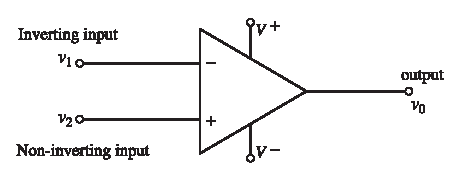
\includegraphics[scale=1.05]{chap4/S3-EE-06-001.eps}
\caption{Circuit symbol of an Op-amp}\label{fig5.1}
\end{figure}

In Fig.~\ref{fig5.1},
\begin{quote}
$v_{1}=$ voltage at the inverting input

$v_{2}=$ voltage at the non-inverting input

$v_{0}=$ output voltage
\end{quote}
All these voltages are measured with respect to ground.

Normally, the Op-amp operates from a bipolar or dual power supply i.e., two power supplies, one positive and one negative with a common ground terminal. The supply voltages are denoted by $V^{+}$ and $V^{-}$ and are in the range $\pm 9$V to $\pm22$V. They are typically $\pm 15$V.

A voltage applied to the non-inverting input produces an in-phase or same polarity voltage at the output while a voltage applied to the inverting input produces an out-of phase or opposite polarity voltage at the output.

The output voltage denoted by $v_{0}$ is proportional to the difference between the input voltages
\begin{equation}
v_{0}=A\,(v_{2}-v_{1})\label{eq5.1}
\end{equation}
where $A$ is the open loop voltage gain.

An Op-amp is basically a differential or difference amplifier, since it amplifies the difference between the applied input signals.

\subsection{Operation of an Op-amp}\label{sec5.1.2}
\index{Operational amplifier!operation of}

The Op-amp is basically a differential amplifier which amplifies the difference between its two input voltages
\begin{equation}
v_{0}=A \ v_{d}=A(v_{2}-v_{1})\label{eq5.2}
\end{equation}
where, $v_{d}=v_{2}-v_{1}=$ difference or differential input voltage
\begin{quote}
$A=$ open loop voltage gain.
\end{quote}

When a voltage $v_{1}$ is applied to the inverting input with the non-inverting input grounded $(v_{2}=0)$ the output voltage is
\begin{equation}
v_{0}=A(v_{2}-v_{1})=A(0-v_{1})=-Av_{1}\label{eq5.3}
\end{equation}

This indicates that the output voltage will be inverted (phase or polarity reversed) with respect to the input voltage.

On the other hand, when a voltage $v_{2}$ is applied to the non-inverting input with the inverting input grounded $(v_{1}=0)$ the output is
\begin{equation}
v_{0}=A(v_{2}-0)=Av_{2}\label{eq5.4}
\end{equation}
which indicates that the output voltage will have the same phase or polarity as the input voltage.

The above facts are illustrated in Fig.~\ref{fig5.2}.
\begin{figure}[H]
\centering
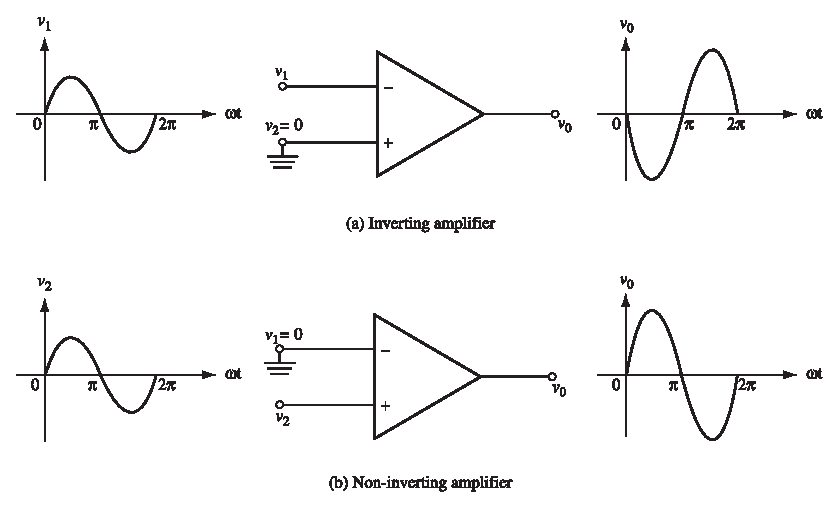
\includegraphics{chap4/S3-EE-06-002.eps}
\caption{Basic operation of an Op-amp}\label{fig5.2}
\end{figure}

\subsection{Properties of an ideal Op-amp}\label{sec5.1.3}

The following are the properties of\index{Operational amplifier!properties of}\index{Ideal Op-amp!properties of} an ideal Op-amp.\index{Ideal Op-amp}\index{Operational amplifier!ideal op-amp}
\begin{enumerate}
\item An ideal Op-amp does not draw any current from the voltage sources connected to its input terminals. Thus its input resistance is infinite, i.e., $R_{i}=\infty$.

\item The output voltage of an ideal Op-amp is independent of the current drawn from it. This means that it has zero output resistance, i.e., $R_{0}=0$.

\item The voltage gain of an ideal Op-amp is infinite, $A=\infty$. This implies that, for a given output voltage, the differential input voltage is essentially zero.

\item An ideal Op-amp amplifies signals of any frequency with a constant gain, which implies that it has an infinite bandwidth, $BW=\infty$.

\item When equal voltages are applied to both the inputs of an ideal Op-amp, its output voltage is zero. Thus, it has a perfect balance.

\item The common-mode rejection ratio of an ideal Op-amp is infinite, i.e., CMRR $=\infty$.

\item An ideal Op-amp has infinite slew-rate, i.e., SR = $\infty$. This implies that the output voltage changes simultaneously with the input voltage.

\item The characteristics of an ideal Op-amp do not change with temperature.

\item The supply voltage or power supply rejection ratio of an ideal Op-amp is zero, i.e., PSRR~=~0.
\end{enumerate}

\subsection{Properties of a practical Op-amp}\label{sec5.1.4}
\index{Operational amplifier!properties of}\index{Practical Op-amp!properties of}\index{Practical Op-amp}\index{Operational amplifier!practical op-amp}

Practical or non-ideal Op-amps differ from the ideal one. Typical characteristics of the practical Op-amps are
\begin{enumerate}
\item The open-loop voltage gain is not infinite, but is generally very high in the range of $10^{4}$ to $10^{6}$ or more.

\item The input resistance is not infinite, but is high and is of the order of megaohms. 

\item The output resistance is not zero, but is of the order of $100\Omega$ or less.

\item The bandwidth is not infinite, but is in the range of 1 to 100 MHz.

\item The common-mode rejection ratio is not infinite, but is of the order of 90 dB.

\item Negative and positive voltage swings (output voltages) are limited by the supply voltages namely, $V^{+}$ and $V^{-}$.
\end{enumerate}

\section{Block diagram of a typical OP-amp}\label{sec5.2}

\vskip -.65cm

\begin{figure}[H]
\centering
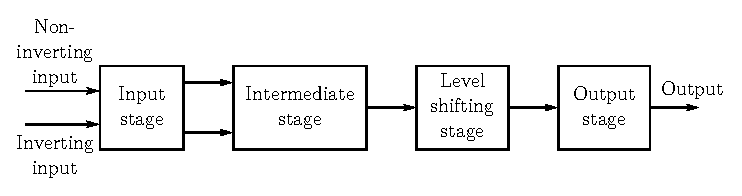
\includegraphics{chap4/fig4.3.eps}
\caption{Block diagram of a Typical Op-amp}\label{addfig5.3}
\end{figure}

Fig.~\ref{addfig5.3} shows the block diagram\index{Operational amplifier!block diagram of} of a typical Op-amp. It consists of the following stages.
\begin{enumerate}
\item Input stage\qquad 2.~ Intermediate stage\qquad 3.~ Level shifting stage\qquad 4. Output stage
\end{enumerate}

Input stage is a Dual-input, balanced output differential amplifier. Dual input means, it can handle two inputs. Balanced output means, the output is zero when the two inputs are equal or set to zero. It provides most of the gain of Op-amp and decides the input impedance of Op-amp.

Intermediate stage is Dual-input, unbalanced output amplifier. Unbalanced output means, the output is nonzero when the two inputs are equal. Intermediate stage contains one or more differential amplifiers to achieve higher differential gain.

The level shifing stage, is usually a CC configuration, used to shift the dc level at the output of the intermediate stage down ward to zero with respect to ground. Due to direct coupling, the dc level of input stage gets coupled to the intermediate stage, resulting in the shift of the operating point. Level translator is used to bring the added dc level to zero without which the output voltage may be distorted.

The output stage is basically a power amplifier that is used to increase the output current supplying capability of the Op-amp. It decides the output impedance of Op-amp. It is desirable to have very low output impedance.

\subsection[Integrated circuit Op-amp ($\mu$A741)]{Integrated circuit Op-amp (\boldmath$\mu$A-741)}\label{sec5.1.5}
\index{Op-amp ($\mu$A-741)}\index{Operational amplifier!op-amp ($\mu$A-741)}

An integrated circuit (IC) is an electronic circuit (or system) in which all the components such as transistors, resistors etc. are fabricated and interconnected during the manufacturing process on a single piece of Silicon wafer called a chip.

A very popular and widely used IC version of Op-amp is $\mu A741$ which is a 8 pin IC available in dual-in-line package or DIP package. The pin diagram of\index{Op-amp ($\mu$A-741)!pin diagram of} $\mu A741$ is shown in Fig.~\ref{fig5.3}.

Pins 1 and 5 are used to null or balance the offset voltages. Offset voltage is the output voltage that occurs even when both the input voltages are zero.

Pin 2 is the inverting input terminal and pin 3 is the non-inverting input terminal.

\vfill\eject

Pins 4 and 7 are the supply voltage pins. The positive supply, $V^{+}$ is connected to pin 7 and the negative supply voltage, $V^{-}$ is connected to pin 4.

Pin 8 is a dummy pin to which no connection is made.
\begin{figure}[H]
\centering
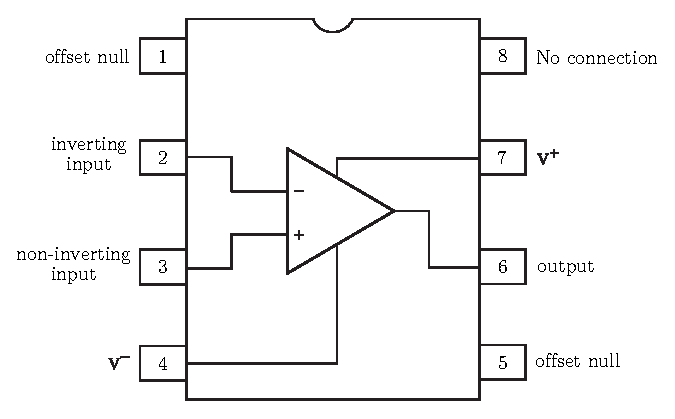
\includegraphics[scale=.9]{chap4/S3-EE-06-003.eps}
\caption{Pin diagram of \ IC 741}\label{fig5.3}
\end{figure}

\subsection[Typical values of various Op-amp parameters for $\mu A741$ IC]{Typical values of various Op-amp parameters for \boldmath$\mu A741$ IC}\label{sec5.1.6}

Table~\ref{tab5.1} lists the typical values of various parameters\index{Op-amp ($\mu$A-741)!parameters} for $\mu A741$ IC. For the purpose of comparison, the ideal values of these parameters are also mentioned.
\begin{table}[H]
\centering
\caption{Typical parameter values for $\mu A741$ IC.}\label{tab5.1}
\renewcommand{\arraystretch}{1}
\begin{tabular}{|r|l|c|c|c|}
\hline
 & & & & {\bf Typical value}\\
{\bf Sl. No.} & \multicolumn{1}{c|}{\bf Parameter} & {\bf Symbol} & {\bf Ideal value} & {\bf for \boldmath$\mu A741$}\\
\hline
1. & Open-loop voltage gain & $A$ & $\infty$ & $2\times 10^{5}$\\
\hline
2. & Input resistance & $R_{i}$ & $\infty$ & 2M$\Omega$\\
\hline
3. & Output resistance & $R_{o}$ & $0$ & $75\Omega$\\
\hline
4. & Input offset current & $I_{io}$ & $0$ & 20\,nA\\
\hline
5. & Input Bias current & $I_{B}$ & $0$ & 80\,nA\\
\hline
6. & Input offset voltage & $V_{io}$ & $0$ & 2\,mV\\
\hline
7. & Common-mode rejection ratio & CMRR, $\rho$ & $\infty$ & 90\,dB\\
\hline
8. & Bandwidth & BW & $\infty$ & 1 MHz\\[-3pt]
   &           &    &          & (at unity gain)\\
\hline
9. & Slew-rate & SR & $\infty$ & 0.5 $V/\mu$S\\
\hline
10. & Power supply rejection ratio & PSRR & $0$ & $30\,\mu$V/V\\
\hline
\end{tabular}
\end{table}

\noindent
{\bf Note:}
\begin{itemize}
\item {\bf Input offset voltage \boldmath$(v_{i0})$}

It is the differential input voltage to be applied to make $v_{0}=0$.

\item {\bf Input Bias current \boldmath$(I_{B})$}

Input bias current, $I_{B}$ is given by
$$
I_{B}=\frac{I_{B_{1}}+I_{B_{2}}}{2}\quad\text{when}\quad v_{0}=0
$$
\end{itemize}

$I_{B_{1}}$ and $I_{B_{2}}$ are the bias currents flowing into the input terminals of Op-amp.

\subsection{Equivalent circuit of an Op-amp}\label{sec5.1.7}

Fig.~\ref{fig5.4} shows the equivalent circuit of\index{Operational amplifier!equivalent circuit of} an Op-amp. Here $R_{i}$ represents the input resistance, measured between the input terminals. It is also called the differential input resistance. The differential input voltage $v_{d}=v_{2}-v_{1}$, is multiplied by the open-loop voltage gain $A$ and appears as $Av_{d}$ at the output. $R_{0}$ represents the output resistance. Note that the output of the Op-amp is represented by a voltage source of value $Av_{d}$ in series with a resistance $R_{o}$.
\begin{figure}[H]
\centering
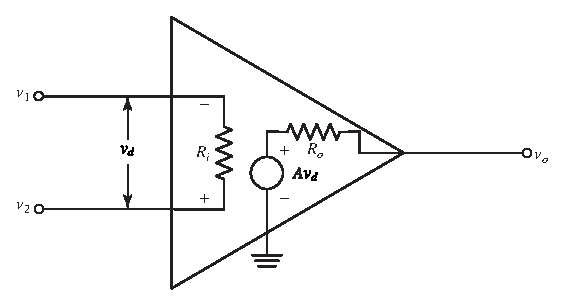
\includegraphics{chap4/S3-EE-06-005.eps}
\caption{Equivalent circuit of the Op-amp}\label{fig5.4}
\end{figure}

\section{Necessity of negative feedback in an Op-amp amplifier}\label{sec5.3}

A practical amplifier is required to amplify a wide band of frequencies with a constant gain i.e., its bandwidth should be very large. For $\mu A741$ IC Op-amp the open loop voltage gain $A$ is $2\times 10^{5}$ and the bandwidth is only 5\,Hz. An amplifier with a high gain and very small bandwidth is practically of no use. For an amplifier the product of voltage gain and bandwidth called the gain-bandwidth product is a constant. Therefore the bandwidth can be increased by reducing the voltage gain. Reduction in voltage gain can be accomplished through negative feedback.

For $\mu A741$, the open loop gain-bandwidth product is
$$
A\times {\rm BW} = (2\times 10^{5})\times 5=10^{6}
$$

Even after incorporating negative feedback,\index{Operational amplifier!negative feedback} the gain bandwidth product should remain the same.
\begin{align}
\text{i.e.,}\qquad A_{f}\times BW_{f} &= 10^{6}\notag\\[3pt]
\Rightarrow\quad A_{f} &= \frac{10^{6}}{BW_{f}}\label{eq5.5}
\end{align}
where,
\begin{quote}
$A_{f}=$ closed loop voltage gain or voltage gain with feedback.

$BW_{f}=$ bandwidth with feedback.
\end{quote}

For example, if a bandwidth of 100\,kHz is required for a given application then the closed loop voltage gain should be
$$
A_{f}=\frac{10^{6}}{100\times 10^{3}}=10
$$
In addition to increase in bandwidth, negative feedback also has the following advantages:
\begin{itemize}
\item[(i)] Amplifier becomes more linear.

\item[(ii)] Input and output impedances are modified towards their ideal values.

\item[(iii)] Voltage gain of the amplifier becomes stable i.e., it becomes independent of Op-amp parameters.
\end{itemize}

\section{Typical frequency response of an Op-amp and the effect of negative feedback on bandwidth of the Op-amp}\label{sec5.3}

The typical frequency response of\index{Operational amplifier!frequency response of} an Op-amp is shown in Fig.~\ref{fig5.5}. This is a plot of open-loop gain versus the frequency. As shown, the gain is approximately constant at $A(=10^{5}\text{~ or~ }100\,\text{dB})$ from 0\,Hz (dc) to a frequency denoted by $f_{i}$. At the frequency $f_{i}$, called the break frequency, the gain is 3\,dB less than its value at 0\,Hz. Beyond $f_{i}$, the open-loop gain decreases at a constant rate of 20\,dB per decade.

\eject

From Fig.~\ref{fig5.5}, for a gain of $10^{5}$ or 100\,dB, the bandwidth is approximately 10\,Hz or the gain bandwidth product is
$$
\text{GBW}=10^{5}\times 10\,{\rm Hz}=1\,\text{MHz}
$$
\begin{figure}[H]
\centering
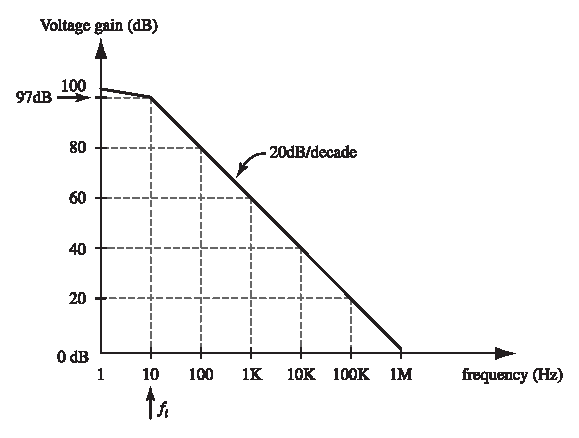
\includegraphics[scale=1.1]{chap4/S3-EE-06-007.eps}
\caption{Frequency response of an Op-amp}\label{fig5.5}
\end{figure}

Since the gain-bandwidth product of an amplifier is a constant, for a gain of unity or 0\,dB the bandwidth is
$$
\frac{\text{GBW}}{\text{Gain}}=\frac{\text{1MHz}}{1}=1\text{MHz}
$$

The frequency at which the gain is unity or 0\,dB is known as the unity gain-bandwidth product (UGB) or simply the bandwidth of an Op-amp. We can write
\begin{equation}
\text{UGB}=Af_{i}\label{eq5.6}
\end{equation}
where
\begin{quote}
$A=$ open loop voltage gain of the Op-amp, called the low frequency gain.

$f_{i}=$ break frequency of the Op-amp.
\end{quote}

\eject

In the presence of negative feedback. 
\begin{equation}
\text{UGB}=A_{f}f'_{i}\label{eq5.7}
\end{equation}
where
\begin{quote}
$A_{f}=$ gain with feedback or closed loop voltage gain.

$f'_{i}=$ bandwidth with feedback.
\end{quote}

From Eqns.~\eqref{eq5.6} and \eqref{eq5.7}
\begin{align}
Af_{i} &= A_{f}f'_{i}\notag\\[4pt]
\text{or}\qquad f'_{i} &= \frac{Af_{i}}{A_{f}}\label{eq5.8}
\end{align}

We know that for a negative feedback amplifier
\begin{equation}
A_{f}=\frac{A}{1+A\beta}\label{eq5.9}
\end{equation}

Substituting Eqn.~\eqref{eq5.9} in Eqn.~\eqref{eq5.8}, we get
\begin{equation}
f'_{i}=\frac{A\cdot f_{i}}{\left(\frac{A}{1+A\beta}\right)}=f_{i}\,(1+A\beta)\label{eq5.10}
\end{equation}

Since $1+A\beta>1$, the bandwidth $f'_{i}>f_{i}$, which means that negative feedback increases the bandwidth.

\smallskip
\noindent
{\bf Note:}~In Fig.~\ref{fig5.5} the gain falls by 20\,dB when frequency increases from 10\,Hz to 100\,Hz or 100\,Hz to 1\,kHz. Ten fold increase in frequency is called a decade. The rate of fall of gain is said to be 20\,dB per decade.

\section{Slew-rate of an Op-amp and its significance}\label{sec5.4}

The slew-rate\index{Slew-rate} or maximum slew-rate of\index{Operational amplifier!slew-rate of} the Op-amp is defined as the maximum time rate of change of its output voltage, expressed in volts per microsecond.
\begin{equation}
\text{SR~ or~ MSR} =\frac{dv_{o}}{dt}\big|_{\max} \ V/\mu \text{\,s}\label{eq5.11}
\end{equation}

Slew-rate is a measure of how fast the Op-amp's output can change in response to changes in the input signal. Hence it limits the maximum operating frequency of the Op-amp. If the frequency of the input signal exceeds a particular value then the output will not be able to follow the input faithfully and the output waveform will be distorted. The output in such situations is referred to as the slew-rate limited output. Fig.~\ref{fig5.6} illustrates such a situation.
\begin{figure}[H]
\centering
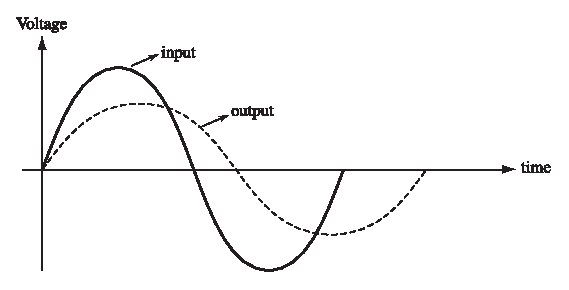
\includegraphics[scale=1.2]{chap4/S3-EE-06-008.eps}
\caption{Effect of slew-rate}\label{fig5.6}
\end{figure}

The slew-rate depends on many factors such as load capacitance. The typical value of the slew-rate for $\mu A741$ IC is 0.5 V/$\mu$\,s. This means that a 10\,V output change from $\mu A741$ typically requires a minimum time of
$$
\text{t}=\frac{10\text{\,V}}{0.5\text{\,V/}\mu\text{\,s}}=20\,\mu\text{\,s}
$$

\smallskip

\begin{example}\label{exam5.1}
Show that the maximum frequency of a sinusoidal voltage that results in an undistorted output from an Op-amp is given by
$$
f_{\max}=\frac{\text{SR}}{2\pi V_{m}}
$$
where SR = maximum slew-rate of the Op-amp.
\end{example}

\begin{solution}
Let the undistorted output signal be represented by
$$
v_{o}=V_{m}\cos \omega t
$$

A cosine wave is considered for convenience.
\begin{align*}
\therefore\quad \dfrac{dv_{o}}{dt}=-\omega V_{m}\sin \omega t\\[3pt]
\text{or}\quad \left|\frac{dv_{o}}{dt}\right|_{\max} &= \omega V_{m}
\end{align*}

\eject

At its maximum $\sin \omega t=1$.

For an undistorted sinusoidal output we require
\begin{align*}
\left|\frac{dv_{o}}{dt}\right|_{\max} &\leq \text{SR}\\[6pt]
\text{i.e.,}\quad \omega V_{m} &\leq \text{SR}\\[6pt]
\text{or}\quad 2\pi fV_{m} &\leq \text{SR}\\[6pt]
\text{or}\quad f &\leq \frac{\text{SR}}{2\pi V_{m}}
\end{align*}

Hence,
\begin{equation}
f_{\max}=\frac{\text{SR}}{2\pi V_{m}}\label{eq5.12}
\end{equation}
\vskip -.7cm
\end{solution}

\begin{example}\label{exam5.2}
If the MSR of an Op-amp is $3V/\mu\text{\,s}$ and the maximum output voltage swing is $\pm 12 V$, calculate the maximum frequency at which the output is a faithful reproduction of the input.
\end{example}

\begin{solution}
Given \ $\text{SR\,}=3V/\mu\text{\,s}$, \ $V_{m}=12\text{\,V}$
\begin{align*}
\text{SR} &=3V/\mu\text{\,s}\\[3pt]
&=3\times 10^{6}V/\text{s}\\[3pt]
f_{\max} &=\frac{\text{SR}}{2\pi V_{m}}\\[3pt]
&=\frac{3\times 10^{6}}{2\pi \times 12}=39.8\text{~kHz}
\end{align*}
\vskip -1cm
\end{solution}

\begin{example}\label{exam5.3}
The output signal of an Op-amp with a slew-rate of 2 V/$\mu$\,s has a maximum value of 10\,V. Find the maximum frequency for undistorted output voltage.
\end{example}

\begin{solution}
Given \ $\text{SR}\,=2V/\mu\text{\,s}=2\times 10^{6}$, \ $V_{m}=10V$.
$$
f_{\max}=\frac{\text{SR}}{2\pi V_{m}}=\frac{2\times 10^{6}}{2\pi\times 10}=31.8\text{~kHz}
$$
\vskip -1cm
\end{solution}

\eject

\section{Common-mode rejection ratio or CMRR of an Op-amp and its significance}\label{sec5.5}

The common-mode rejection ratio\index{Common-mode rejection ratio} or CMRR\index{Operational amplifier!CMRR} is a figure of merit or performance measure of an Op-amp. It is defined as the ratio of the differential gain, $A_{d}$, to the common-mode gain, $A_{c}$.
\begin{equation}
\text{CMRR}=\rho=\frac{|A_{d}|}{|A_{c}|}\label{eq5.13}
\end{equation}
CMRR is more often expressed in decibels as
\begin{equation}
\text{CMRR}=20\log_{10}\left|\frac{A_{d}}{A_{c}}\right|\text{\,dB}\label{eq5.14}
\end{equation}
The typical value of CMRR for $\mu A741$ IC Op-amp is 90\,dB.

For an ideal Op-amp $A_{d}$ is infinite and $A_{c}$ is zero so that CMRR is infinite. However, for a practical Op-amp $A_{d}$ is very large and $A_{c}$ is non-zero but small, so that CMRR is very large.

The common-mode rejection ratio is a measure of the ability of the Op-amp to reject signals common to both the inputs i.e., its ability to produce a zero output voltage when both the inputs are exactly identical.

It is advantageous to use Op-amps with large CMRR as they have better ability to reject noise signals such as 50\,Hz power line hum which are common to both the inputs.

\smallskip

\begin{example}\label{exam5.4}
An Op-amp has a differential gain of 500 and a CMRR of 80\,dB. If the common-mode input signal is $2\sin 100\pi t$V, calculate the common-mode output voltage.
\end{example}

\begin{solution}
\begin{align*}
\text{CMRR~ in~ dB~ } &= 20\log \frac{|A_{d}|}{|A_{c}|}\\[5pt]
\text{i.e.,}\quad 80\text{\,dB} &= 20\log \frac{|A_{d}|}{|A_{c}|}\\[5pt]
\text{or}\quad \frac{A_{d}}{A_{c}} &= \text{antilog}\left(\frac{80}{20}\right)=\text{antilog (4)}\\[5pt]
\therefore\quad \frac{A_{d}}{A_{c}} &= 10000\\[5pt]
\text{or}\quad A_{c} &= \frac{A_{d}}{10000}=\frac{500}{10000}=0.05
\end{align*}

\eject

Therefore, the common-mode output voltage is
\begin{align*}
A_{c}V_{c} &= 0.05\times 2\sin 100\pi t\text{~V}\\[4pt]
&= 0.1\sin 100\pi t\text{~V}
\end{align*}
\vskip -.7cm
\end{solution}

\begin{example}\label{exam5.5}
An Op-amp has an open loop voltage gain of $10^{4}$ and a common-mode voltage gain of 0.1. Express its CMRR in dB.
\end{example}

\begin{solution}
Given \ $A_{d}=A=10^{4}$, \ $A_{c}=0.1$
\begin{align*}
\text{CMRR} &= 20\log \frac{|A_{d}|}{|A_{c}|}=20\log \left(\frac{10^{4}}{0.1}\right)\\[4pt]
&= 20\log (10^{5})=100\text{\,dB}
\end{align*}
\vskip -.7cm
\end{solution}

\begin{example}\label{exam5.6}
Show that the output of a differential amplifier can be expressed as
$$
v_{0}=A_{d}v_{d}\left[1+\frac{1}{\rho}v_{c}\right]
$$
\end{example}

\begin{solution}
Fig.~(A) shows a differential amplifier with input voltages $v_{1}$ and $v_{2}$ and output voltage $v_{0}$.
\begin{figure}[H]
\centering
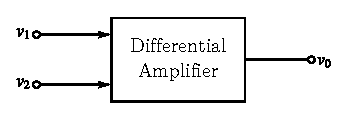
\includegraphics{chap4/sol4.6.eps}

\medskip
\colorbox{lightgray}{\bf Fig.~(A)}
\end{figure}

For a linear differential amplifier, $v_{0}$ can be expressed as a linear combination of $v_{1}$ and $v_{2}$.
\begin{equation*}
v_{0}=A_{1}v_{1}+A_{2}v_{2}\tag{A}
\end{equation*}

The differential input voltage is given by
\begin{equation*}
v_{d}=v_{2}-v_{1}\tag{B}
\end{equation*}

The common mode input voltage is given by
\begin{equation*}
v_{c} = \frac{v_{1}+v_{2}}{2}\tag{C}
\end{equation*}

\eject

Solving Eqns.~(B) and (C), we obtain
\begin{align*}
v_{1} &= v_{c}-\frac{1}{2}v_{d}\tag{D}\\[3pt]
v_{2} &= v_{c}+\frac{1}{2}v_{d}\tag{E}
\end{align*}

Substituting Eqns.~(D) and (E) in Eqn.~(A), we have
\begin{align*}
v_{0} &= A_{1}\left[v_{c}-\frac{1}{2}v_{d}\right]+A_{2}\left[v_{c}+\frac{1}{2}v_{d}\right]\\[4pt]
\text{or}\qquad v_{0} &= \frac{[A_{2}-A_{1}]}{2}v_{d}+[A_{1}+A_{2}]v_{c}\tag{F}
\end{align*}

Taking, $A_{d}=\dfrac{A_{2}-A_{1}}{2}$ and $A_{c}=A_{1}+A_{2}$, we have
\begin{equation*}
v_{0}=A_{d}v_{d}+A_{c}v_{c}\tag{G}
\end{equation*}
where, 
\begin{align*}
A_{d} &= \text{Differential gain}\\[3pt]
A_{c} &= \text{Common mode gain}\\[3pt]
\therefore\qquad v_{0} &=A_{d}v_{d}\left[1+\frac{A_{c}}{A_{d}}\frac{v_{c}}{v_{d}}\right]\tag{H}
\end{align*}

But,
$$
\text{CMRR}=\rho =\dfrac{A_{d}}{A_{c}}\Rightarrow \frac{1}{\rho}=\frac{A_{c}}{A_{d}}
$$
Using this relation in Eqn.~(H), we have
\begin{equation*}
v_{0}=A_{d}v_{d}\left[1+\frac{1}{\rho}\frac{v_{c}}{v_{d}}\right]\tag{I}
\end{equation*}

Note that, as $\rho\to \infty$
$$
v_{0}\to A_{d}v_{d}
$$
which is a highly desirable characteristic of a differential amplifier.
\end{solution}

\section{Concept of virtual short in an Op-amp}\label{sec5.6}
\index{Virtual short}

Fig.~\ref{fig5.7} shows the circuit of Op-amp inverting amplifier which employs negative feedback.
\begin{figure}[H]
\centering
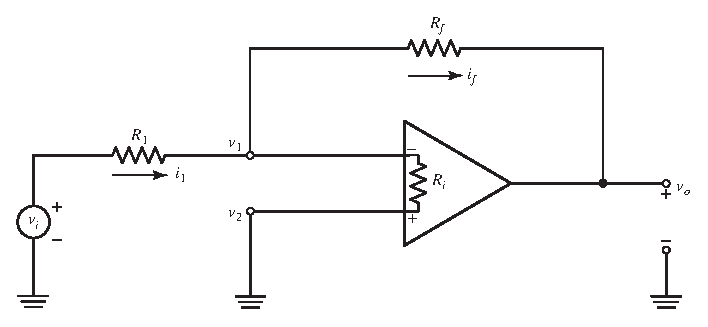
\includegraphics{chap4/S3-EE-06-011.eps}
\caption{Op-amp inverting amplifier with negative feedback}\label{fig5.7}
\end{figure}

\noindent
$R_{i}$ represents the input resistance of Op-amp measured between the inverting and non-inverting input terminals. The output voltage $v_{o}$ is given by
\begin{align}
v_{0} &= A\,[v_{2}-v_{1}]\qquad
\text{or}\qquad v_{2}-v_{1} = \frac{v_{0}}{A}\label{eq5.15}
\end{align}
where $A$ is the open loop voltage gain of Op-amp.

\smallskip

The output voltage $v_{o}$ cannot exceed the DC supply voltage given to the Op-amp. For $\mu A741$, typical supply voltage is 12\,V and the open loop voltage gain $A$ is $2\times 10^{5}$. To get an output voltage of 10\,V, the required differential input voltage is
$
v_{2}-v_{1}=\dfrac{10\,\text{V}}{2\times 10^{5}}=0.5\,\mu\text{\,V}.
$

\smallskip

This value is very small compared to the input and output voltages and may be considered as 0\,V.
\begin{align}
\text{i.e.,}\quad v_{2}-v_{1} &\simeq 0\,\text{V}\qquad
\text{or}\qquad v_{2} = v_{1}\label{eq5.16}
\end{align}
From Eqn.~\eqref{eq5.16} we find that the inverting and non-inverting input terminals are at the same potential i.e., they appear to be tied together or shorted. Therefore voltage across $R_{i}$ is zero.

Further since $R_{i}$ is very large $[2\text{~M}\Omega\text{~~ for~~ }\mu A741]$ the current flowing through $R_{i}$ is almost zero. Thus the voltage across $R_{i}$ and the current through $R_{i}$ are both zero.

If two terminals are physically shorted, the voltage between the two terminals will be zero and a large current flows through this short. Since the voltage between the input terminals is zero and no current flows through the short to the ground, we say that a virtual short\index{Operational amplifier!virtual short} exists between the input terminals of Op-amp. The virtual short is also called the virtual ground. The virtual ground is indicated by thick line between the input terminals as shown in Fig.~\ref{fig5.8}.
\begin{figure}[H]
\centering
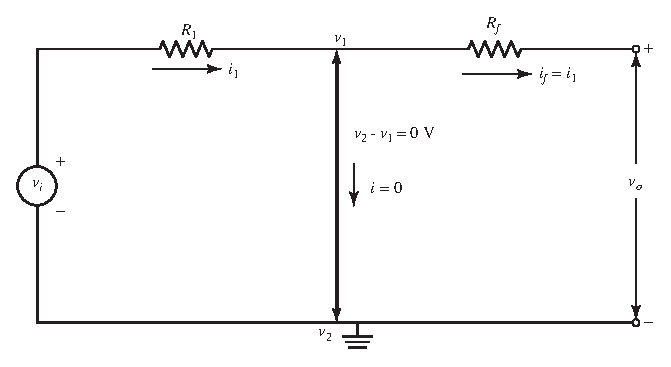
\includegraphics{chap4/S3-EE-06-012.eps}
\caption{Virtual ground in Op-amp}\label{fig5.8}
\end{figure}
Note that same current flows through $R_{1}$ and $R_{f}$. The concept of virtual short is very much usefull in the analysis of Op-amp circuits.

\section{Basic Op-amp circuits}\label{addsec5.8}
\index{Op-amp circuits}

The basic Op-amp circuits\index{Operational amplifier!basic Op-amp circuits} are
\begin{itemize}
\item[(a)] Inverting amplifier.\qquad\quad 
(b)~ Non inverting amplifier.
\end{itemize}
These circuits are discussed in the following sections. 

\section{Op-amp inverting amplifier}\label{sec5.7}

Fig.~\ref{fig5.9} shows the circuit of an Op-amp inverting amplifier.\index{Inverting amplifier}\index{Op-amp circuits!inverting amplifier}\index{Operational amplifier!inverting amplifier} The input signal $v_{i}$ is applied to the inverting input terminal through the resistor $R_{1}$ and the non-inverting input terminal is grounded. Feed back from output to the inverting input terminal is provided through the feedback resistor $R_{f}$. Since the input is applied to the inverting input terminal, $v_{o}$ and $v_{i}$ are of opposite polarity and hence the feedback is negative. Since the non-inverting input terminal is grounded, $v_{2}=0$. Due to the virtual short at the input of Op-amp, the inverting and non-inverting input terminals are at the same potential.
$$
\therefore\quad v_{1}=v_{2}=0
$$
\vskip -.65cm
\begin{figure}[H]
\centering
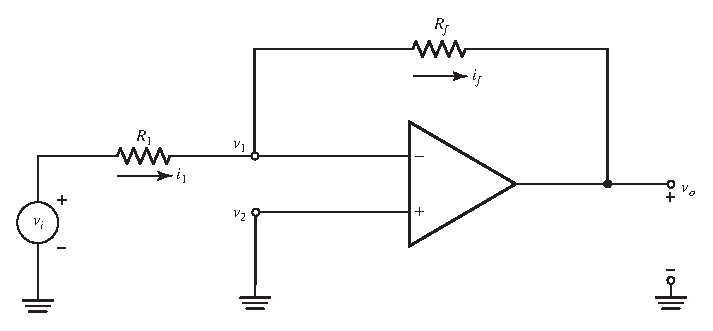
\includegraphics{chap4/S3-EE-06-013.eps}
\caption{Op-amp inverting amplifier}\label{fig5.9}
\end{figure}

\noindent
Due to high input impedance of the Op-amp, the current flowing into its inverting input terminal is zero. Therefore, same current flows through $R_{1}$ and $R_{f}$
\begin{align}
\text{i.e.,}\quad i_{1} &= i_{f}\label{eq5.17}\\[3pt]
\text{But}\quad i_{1} &= \frac{v_{i}-v_{1}}{R_{1}}=\frac{v_{i}}{R_{1}}\label{eq5.18}\\[3pt]
\text{and}\quad i_{f} &= \frac{v_{1}-v_{0}}{R_{f}}=-\frac{v_{0}}{R_{f}}\label{eq5.19}
\end{align}
Using these relations in Eqn.~\eqref{eq5.17} we have
\begin{align}
\frac{v_{i}}{R_{1}} &=-\frac{v_{0}}{R_{f}}\notag\\[3pt]
A_{f}=\frac{v_{0}}{v_{i}} &= -\frac{R_{f}}{R_{1}}\label{eq5.20}
\end{align}
$A_{f}$ is the closed loop voltage gain or voltage gain with negative feedback.

Note that $A_{f}$ depends only on the external resistors $R_{f}$ and $R_{1}$. The negative sign implies that $v_{o}$ and $v_{i}$ are of opposite polarity.

\eject

\begin{example}\label{exam5.6}
A 200\,mV peak to peak sine waveform voltage is applied to an Op-amp inverting amplifier with $\dfrac{R_{f}}{R_{1}}=10$. Sketch the output.
\end{example}

\begin{solution}
Peak to peak input voltage,
\begin{align*}
2\,V_{m} &= 200\text{\,mV}\\[4pt]
V_{m} &= 100\text{\,mV}\\[4pt]
\text{input voltage,~ } v_{i} &= V_{m}\sin \omega t=100\sin \omega t\text{~mV}\\[4pt]
v_{0} &= \frac{-R_{f}}{R_{1}}\times v_{i}\\[4pt]
&= -10\times 100\sin \omega t\text{~mV}=-1000\sin \omega t\text{~mV}=-\sin \omega t\text{\,V}
\end{align*}
The input and output voltages are shown below.
\begin{figure}[H]
\centering
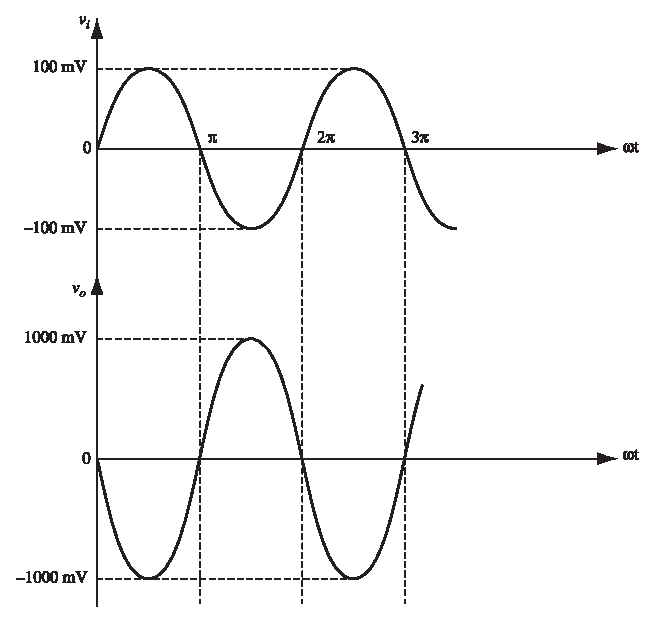
\includegraphics{chap4/S3-EE-06-IN001.eps}

\medskip
{\em observe that $v_{o}$ and $v_{i}$ are $180^{\circ}$ out of phase.}
\end{figure}
\vskip -.7cm
\end{solution}

\eject

\begin{example}\label{exam5.7}
Design an inverting amplifier using Op-amp with a closed loop voltage gain of~$-15$.
\end{example}

\begin{solution}
\begin{align*}
A_{f} &= -15=-\frac{R_{f}}{R_{1}}\\[3pt]
R_{f} &= 15R_{1}
\end{align*}
If we select $R_{1}=1$\,k$\Omega$ then $R_{f}=15\text{k}\Omega$.

The inverting amplifier circuit is shown below
\begin{figure}[H]
\centering
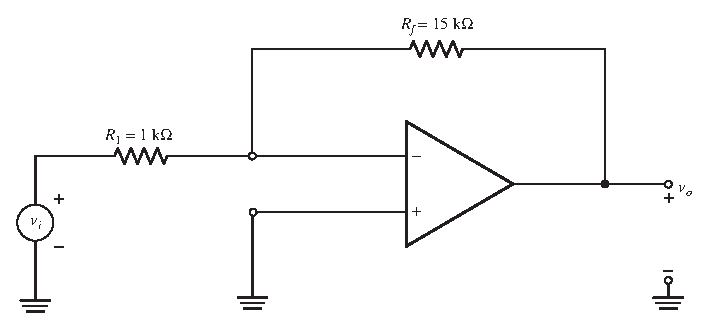
\includegraphics[scale=.95]{chap4/S3-EE-06-IN002.eps}
\end{figure}

\noindent
{\bf Note:}~The gain resistors $R_{1}$ and $R_{f}$ should neither be too large nor too small. Too small value of resistors demand more current from the input source to produce the required voltage drops and too large value of resistors results in insufficient bias currents at Op-amp input. Hence a reasonable range of values would be form a few kilo-ohms to few hundred kilo-ohms.
\end{solution}

\begin{example}\label{exam5.8}
For the circuit shown below calculate the output voltage for the following input voltages.
\begin{itemize}
\item[(i)] $v_{i}=0.2$V\qquad (ii)~ $v_{i}=0.5\sin 314t$V\qquad (iii) $v_{i}=-0.4$V
\end{itemize}
\begin{figure}[H]
\centering
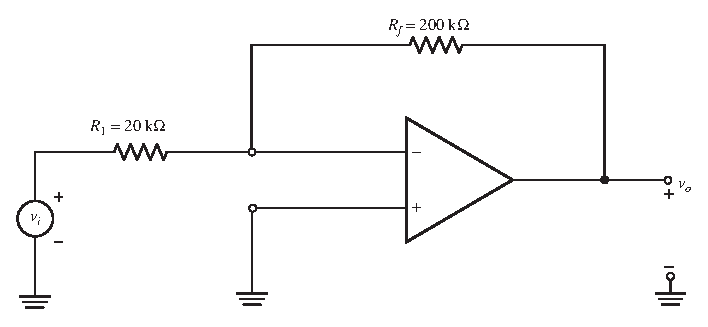
\includegraphics[scale=.95]{chap4/S3-EE-06-IN003.eps}
\end{figure}
\end{example}

\eject

\begin{solution}
\begin{align*}
A_{f} &= -\frac{R_{f}}{R_{1}}\\[3pt]
&=-\frac{200\, k\Omega}{20\, k\Omega} = -10\\[3pt]
A_{f} &= \frac{v_{o}}{v_{i}}\\[3pt]
v_{0} &= A_{f}\,v_{i}=-10\,v_{i}
\end{align*}
\begin{itemize}
\item[(i)]
\begin{tabbing}
$v_{i}$ \== $0.2$\,V\\[3pt]
$v_{o}$ \>= $-10\times 0.2\text{\,V}=-2\text{\,V}$
\end{tabbing}

\smallskip

\item[(ii)]
\begin{tabbing}
$v_{i}$ \== $0.5\sin 314t\,$V\\[3pt]
$v_{o}$ \>= $-10\times 0.5\sin 314t\,$V\\[3pt]
        \>= $-5\sin 314t\,$V
\end{tabbing}

\smallskip

\item[(iii)]
\begin{tabbing}
$v_{i}$ \== $-0.4$\,V\\[3pt]
$v_{o}$ \>= $-10\times -0.4\,$V\\[3pt]
\>= $4\,$V
\end{tabbing}
\end{itemize}
\vskip -.7cm
\end{solution}

\begin{example}\label{exam5.9}
For the circuit shown below calculate the
\begin{itemize}
\item[(i)] Closed loop voltage gain.

\item[(ii)] Required input voltage to get an output voltage of 2V.
\end{itemize}
\begin{figure}[H]
\centering
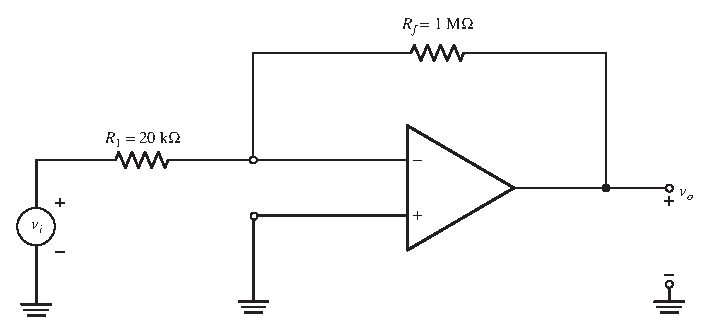
\includegraphics{chap4/S3-EE-06-IN004.eps}
\end{figure}
\end{example}

\eject

\begin{solution}
~

\begin{itemize}
\item[(i)]
\begin{tabbing}
$A_{f}$ \== $\dfrac{-R_{f}}{R_{1}}$\\[9pt]
        \>= $\dfrac{-10^{6}\Omega}{20\times 10^{3}\Omega}$\\[9pt]
        \>= $-50$
\end{tabbing}

\smallskip

\item[(ii)] 
\begin{tabbing}
$A_{f}$ \== $\dfrac{v_{o}}{v_{i}}$\\[8pt]
~\,$v_{i}$ \>= $\dfrac{v_{o}}{A_{f}}$\\[8pt]
        \>= $\dfrac{2\text{\,V}}{-50}$\\[8pt]
        \>= $-\,0.04$\,V
\end{tabbing}
\end{itemize}
\vskip -.7cm
\end{solution}

\begin{example}\label{exam5.10}
For the inverting amplifier circuit shown below find
\begin{itemize}
\item[(i)] Equivalent feedback resistor $R_{f}$.

\item[(ii)] Closed loop voltage gain $A_{f}$.
\end{itemize}
Take $R_{1}=1\, k\Omega$, \ $R_{2}=R_{3}=10\, k\Omega$ \ \ and \ \ $R_{4}=100\Omega$.
\begin{figure}[H]
\centering
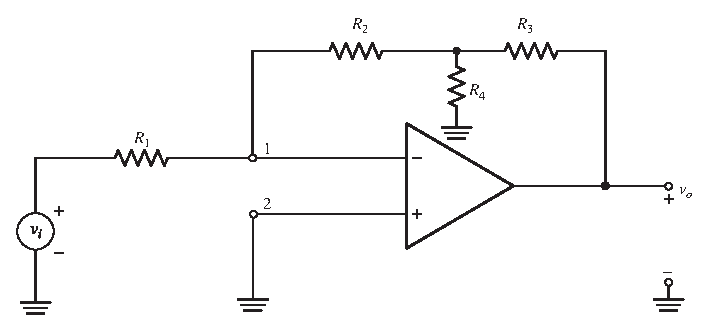
\includegraphics{chap4/S3-EE-06-IN005.eps}
\end{figure}
\end{example}

\eject

\begin{solution}
The inverting amplifier with $R_{f}$ is shown in Fig.~A.
\begin{figure}[H]
\centering
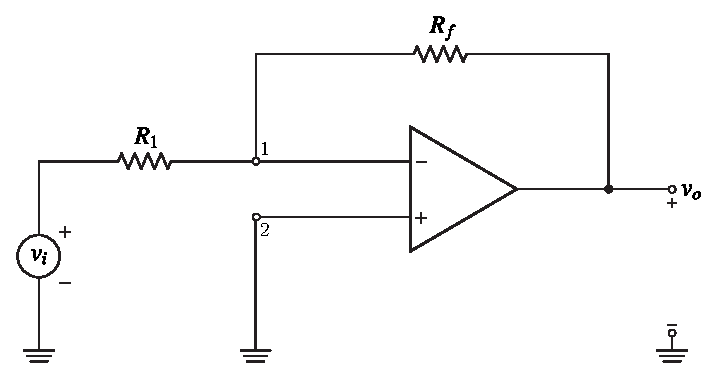
\includegraphics{chap4/S3-EE-06-IN006.eps}

\medskip
\bigskip
\colorbox{lightgray}{\bf Fig. A}
\end{figure}

Due to virtual short at the input of Op-amp, terminals 1 \&\ 2 are shorted to ground as shown in Fig.~B.
\begin{figure}[H]
\centering
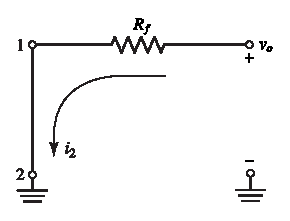
\includegraphics[scale=1.35]{chap4/S3-EE-06-015.eps}

\medskip
\bigskip
\colorbox{lightgray}{\bf Fig. B}
\end{figure}

\noindent
$i_{2}$ is the current flowing into the short between the terminals 1 \&\ 2.
\begin{equation*}
R_{f}=\frac{v_{o}}{i_{2}}\tag{A}
\end{equation*}

\eject

Let us write the equivalent circuit of the given circuit using the concept of virtual short as shown in Fig.~C.
\begin{figure}[H]
\centering
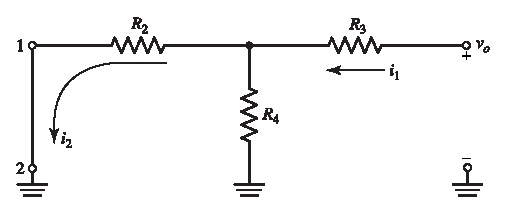
\includegraphics{chap4/S3-EE-06-016.eps}

\medskip
\colorbox{lightgray}{\bf Fig.~C}
\end{figure}
\noindent
$R_{2}$ and $R_{4}$ are in parallel.
\begin{align*}
\text{Let}\qquad R &= R_{2}\, ||\, R_{4}= \frac{R_{2}R_{4}}{R_{2}+R_{4}}\tag{B}
\end{align*}

The simplified circuit is shown in Fig.~D
\begin{figure}[H]
\centering
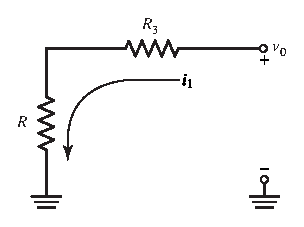
\includegraphics{chap4/S3-EE-06-017a.eps}

\smallskip
\colorbox{lightgray}{\bf Fig. D}
\end{figure}
\begin{equation*}
\text{From Fig.~D},\qquad i_{1}=\frac{v_{o}}{R+R_{3}}\tag{C}
\end{equation*}
Applying current division rule to the circuit of Fig.~C, we have
\begin{align*}
i_{2} &= \frac{i_{1}\,R_{4}}{R_{2}+R_{4}}\\[3pt]
i_{2} &= \frac{v_{o}}{(R+R_{3})}\;\frac{R_{4}}{(R_{2}+R_{4})}\\[3pt]
\frac{v_{o}}{i_{2}} &= \frac{(R+R_{3})(R_{2}+R_{4})}{R_{4}}\tag{D}
\end{align*}
Comparing Eqns.~(A) and (D) we have
\begin{equation*}
R_{f}=\frac{(R+R_{3})(R_{2}+R_{4})}{R_{4}}\tag{E}
\end{equation*}
Substituting for $R$ from Eqn.~(B) we have
\begin{align*}
R_{f} &= \frac{\left(\frac{R_{2}R_{4}}{R_{2}+R_{4}}+R_{3}\right)(R_{2}+R_{4})}{R_{4}}\\[6pt]
&= \frac{R_{2}R_{4}+R_{3}(R_{2}+R_{4})}{R_{4}}\\[6pt]
R_{f} &= R_{2}+R_{3}+\frac{R_{2}R_{3}}{R_{4}}\tag{F}
\end{align*}
Closed loop voltage gain
\begin{align*}
A_{f} &= \frac{-R_{f}}{R_{1}}\\[4pt]
&= \frac{-\left[R_{2}+R_{3}+\frac{R_{2}R_{3}}{R_{4}}\right]}{R_{1}}\tag{G}
\end{align*}
Given $R_{1}=1 k\Omega$, $R_{2}=R_{3}=10 k\Omega$, $R_{4}=100\Omega = 0.1 k\Omega$.

\smallskip

From Eqn.~(F)
\begin{align*}
R_{f} &= 10\, k\Omega +10\, k\Omega +\frac{10\, k\Omega\times 10\, k\Omega}{0.1\, k\Omega}\\[4pt]
&= 1020\, k\Omega
\end{align*}

From Eqn.~(G)
\begin{align*}
A_{f} &= \frac{-1020\, k\Omega}{1\, k\Omega}\\[4pt]
&= -1020
\end{align*}
\vskip -.9cm
\end{solution}

\eject

\section{Op-amp non-inverting amplifier}\label{sec5.8}

Fig.~\ref{fig5.10} Shows the circuit of an Op-amp non-inverting amplifier\index{Non-inverting amplifier}\index{Op-amp circuits!non-inverting amplifier}\index{Operational amplifier!non-inverting amplifier}
\begin{figure}[H]
\centering
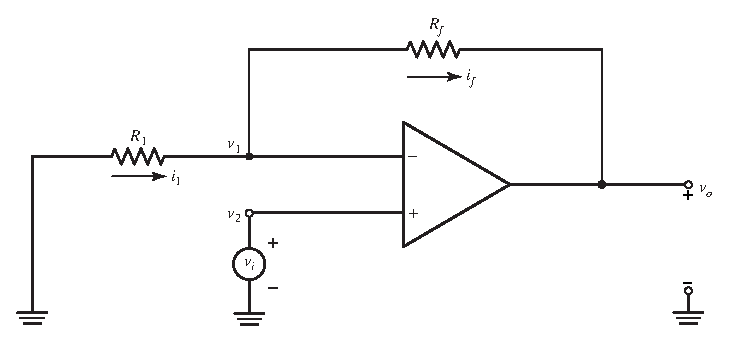
\includegraphics[scale=1.1]{chap4/S3-EE-06-017b.eps}

\smallskip
\caption{}\label{fig5.10}
\end{figure}

Feedback resistor $R_{f}$ appears between the output terminal and inverting input terminal. $R_{1}$ connects the inverting terminal to ground. The input signal $v_{i}$ is applied at the non-inverting input terminal
\begin{equation}
\therefore\quad v_{2}=v_{i}\label{eq5.21}
\end{equation}

Due to virtual short at the input of Op-amp, the inverting and non-inverting input terminals are at the same potential.
\begin{equation}
\therefore\quad v_{1}=v_{2}\label{eq5.22}
\end{equation}
Combining Eqns.~\eqref{eq5.21} and \eqref{eq5.22} we get
\begin{equation}
v_{1}=v_{i}\label{eq5.23}
\end{equation}

Due to high input impedance of Op-amp, the current flowing into its inverting input terminal is zero. As a result same current flows through $R_{1}$ and $R_{f}$.
\begin{equation}
\text{i.e.,}\quad i_{1}=i_{f}\label{eq5.24}
\end{equation}

\eject

But
\begin{align}
i_{1} &= \frac{0-v_{1}}{R_{1}}=\frac{-v_{i}}{R_{1}}\label{eq5.25}\\[5pt]
\text{and}\quad i_{f} &= \frac{v_{1}-v_{o}}{R_{f}}=\frac{v_{i}-v_{o}}{R_{f}}\label{eq5.26}
\end{align}
Using these relations in Eqn.~\eqref{eq5.24} we have
\begin{align}
\frac{-v_{i}}{R_{1}} &= \frac{v_{i}-v_{o}}{R_{f}}\notag\\[5pt]
\frac{v_{o}}{R_{f}} &= v_{i}\left[\frac{1}{R_{1}}+\frac{1}{R_{f}}\right]\notag\\[5pt]
v_{o} &= v_{i}\,R_{f}\left[\frac{R_{f}+R_{1}}{R_{1}R_{f}}\right]\notag\\[5pt]
A_{f} &= \frac{v_{o}}{v_{i}}=1+\frac{R_{f}}{R_{1}}\label{eq5.27}
\end{align}
$A_{f}$ is the closed loop voltage gain or voltage gain with negative feedback. From Eqn.~\eqref{eq5.27} we observe that,
\begin{itemize}
\item[(i)] $A_{f}$ depends only on external resistors $R_{f}$ and $R_{1}$.

\item[(ii)] $A_{f}$ is positive and hence $v_{o}$ and $v_{i}$ are in phase.
\end{itemize}

\begin{example}\label{exam5.11}
Design a non-inverting amplifier using Op-amp with a closed loop voltage gain of 10.
\end{example}

\begin{solution}
Given,
\begin{align*}
A_{f}=1+\frac{R_{f}}{R_{1}} &= 10\\[4pt]
\therefore\quad \frac{R_{f}}{R_{1}} &= 9\\[4pt]
\text{or}\quad R_{f} &= 9R_{1}
\end{align*}
If we select $R_{1}=1 k\Omega$.

Then \ $R_{f}=9 k\Omega$.

\eject

The non-inverting amplifier circuit is shown below.
\begin{figure}[H]
\centering
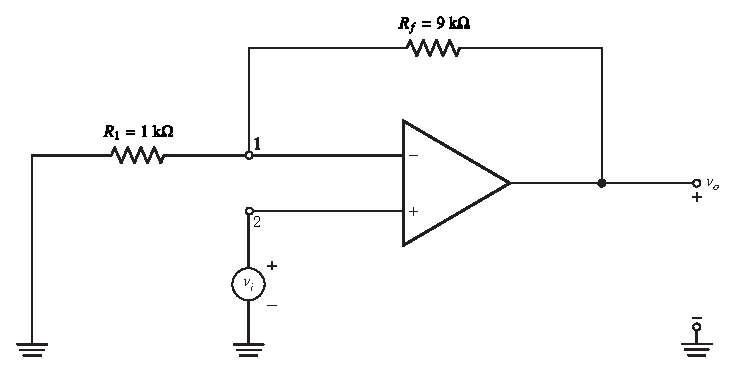
\includegraphics[scale=1.1]{chap4/exp4.12.eps}
\end{figure}
\vskip -.5cm
\end{solution}

\medskip

\begin{example}\label{exam5.12}
For the circuit shown below calculate the output voltage for the following input voltages.
\begin{itemize}
\item[(i)] $v_{i}=0.5\,$V.

\item[(ii)] $v_{i}=0.6\cos (314t)$\,V.

\item[(iii)] $v_{i}={}-0.3\,$V.
\end{itemize}
\begin{figure}[H]
\centering
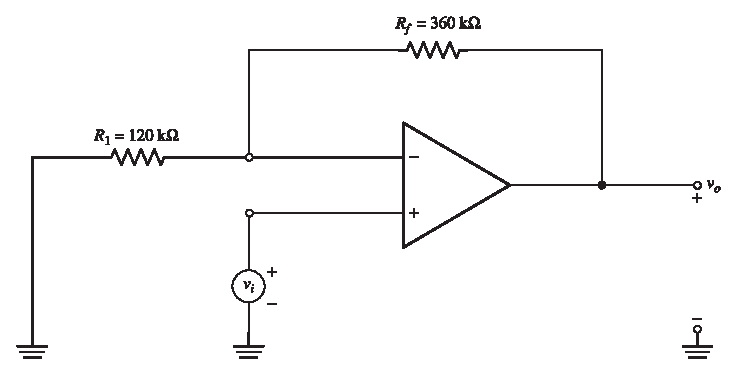
\includegraphics[scale=1.1]{chap4/S3-EE-06-IN007.eps}
\end{figure}
\end{example}

\eject

\begin{solution}
\begin{align*}
A_{f} &= 1+\frac{R_{f}}{R_{1}}\\[3pt]
&= 1+\frac{360\, k\Omega}{120\, k\Omega}\\[3pt]
&=4\\[3pt]
A_{f} &= \frac{v_{o}}{v_{i}}\\[3pt]
v_{o} &= A_{f}\,v_{i}
\end{align*}
\begin{itemize}
\item[(i)]
\begin{tabbing}
$v_{i}$ \== $0.5$\,V\\[3pt]
$v_{o}$ \>= $4\times 0.5\,\text{V}=2\text{\,V}$
\end{tabbing}

\item[(ii)]
\begin{tabbing}
$v_{i}$ \== $0.6\cos 314t\,$V\\[3pt]
$v_{o}$ \>= $4\times 0.6\cos 314t\,$V\\[3pt]
\>= $2.4\cos 314t\,$V
\end{tabbing}

\item[(iii)]
\begin{tabbing}
$v_{i}$ \== ${}-0.3\,$V\\[3pt]
$v_{o}$ \>= $4\times -\,0.3\,$V\\[3pt]
\>= $-1.2\,$V
\end{tabbing}
\end{itemize}
\vskip -.6cm
\end{solution}

\begin{example}\label{exam5.13}
For the circuit shown below calculate
\begin{itemize}
\item[(i)] Closed loop voltage gain.

\item[(ii)] Required input voltage to get an output voltage of 4\,V.

\item[(iii)] Maximum input voltage that can be applied without driving the Op-amp into saturation, if the supply voltage to the Op-amp is, $\pm 12V$.
\end{itemize}
\begin{figure}[H]
\centering
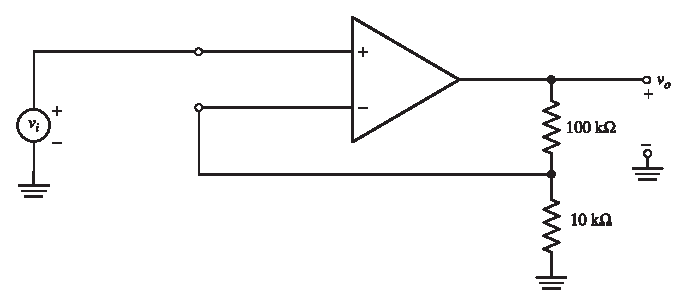
\includegraphics{chap4/S3-EE-06-IN008.eps}
\end{figure}
\end{example}

\begin{solution}
The given circuit is a non-inverting amplifier
\begin{align*}
R_{f} &= 100\, k\Omega\\[3pt]
R_{1} &= 10\, k\Omega
\end{align*}
\begin{itemize}
\item[(i)]
\begin{tabbing}
$A_{f}$ \== $1+\dfrac{R_{f}}{R_{1}}$\\[4pt]
\>= $1+\dfrac{100\, k\Omega}{10\, k\Omega}= 11$
\end{tabbing}

\item[(ii)]
\begin{tabbing}
$A_{f}$ \== $\dfrac{v_{o}}{v_{i}}$\\[4pt]
~\,$v_{i}$ \>= $\dfrac{v_{o}}{A_{f}}= \dfrac{4\,{\rm V}}{11}= 0.364\,$V
\end{tabbing}

\item[(iii)]
The largest obtainable output voltage is limited by the supply voltage
\begin{align*}
\therefore\qquad v_{0}(\max) &= \pm 12V\\[3pt]
\text{Now,}\qquad v_{i}(\max) &= \frac{v_{0}(\max)}{A_{f}}=\frac{\pm 12V}{11}\\[3pt]
&= \pm 1.09V
\end{align*}
\end{itemize}
\vskip -.9cm
\end{solution}

\medskip

\begin{example}\label{exam5.14}
In an Op-amp inverting amplifier $R_{1}=1\,k\Omega$, $R_{f}=100\,k\Omega$. The DC supply voltage to the Op-amp is $\pm 15\,$V. Calculate the output voltage if the input voltage is 1\,V.
\end{example}

\begin{solution}
\begin{align*}
R_{1} &= 1 k\Omega, \ R_{f}=100\,k\Omega\\[4pt]
V^{+} &= 15\,{\rm V}, \ V^{\,-}=-15\text{\,V}, \ v_{i}=1\text{\, V}\\[4pt]
A_{f} &= \frac{-R_{f}}{R_{1}}=\dfrac{-100\,k\Omega}{1\,k\Omega}\\[4pt]
&= -100\\[4pt]
A_{f} &= \frac{v_{o}}{v_{i}}\\[4pt]
v_{o} &= A_{f}\,v_{i}\\[4pt]
&= -100\times 1\text{\,V}\\[4pt]
&= -100\text{\,V}
\end{align*}
The output voltage cannot exceed the DC power supply voltage. Since $v_{o}$ is negative and large it is limited to $V^{\,-}$
$$
\therefore\quad v_{o}\simeq V^{\,-}=-15V
$$
\vskip -.7cm
\end{solution}

\eject

\begin{example}\label{exam5.15}
In an Op-amp non-inverting amplifier $R_{1}=2\,k\Omega$ and $R_{f}=200\,k\Omega$. The DC supply voltage to the Op-amp is $\pm 12\,$V. Calculate the output voltage if the input voltage is 1.5\,V.
\end{example}

\begin{solution}
\begin{align*}
R_{1} &= 2\,k\Omega, \ R_{f}=200\,k\Omega\\[3pt]
V^{+} &= 12\,\text{V}, \ V^{\,-}=-12\,\text{V}, \ v_{i}=1.5\text{\,V}\\[3pt]
A_{f} &= 1+\frac{R_{f}}{R_{1}}\\[3pt]
&= 1+\frac{200\, k\Omega}{2\, k\Omega}\\[3pt]
&= 101\\[3pt]
v_{o} &= A_{f}\,v_{i}\\[3pt]
&= 101\times 1.5 \text{\,V}\\[3pt]
&= 151.5\text{\,V}
\end{align*}
The output voltage cannot exceed the DC power supply voltage. Since, $v_{o}$ is positive and large, it is limited to $V^{+}$
$$
\therefore\quad v_{o}\simeq V^{+}=12\text{\,V}
$$
\vskip -.7cm
\end{solution}

\section{Expression for input resistance of Op-amp inverting amplifier}\label{sec5.9}


Fig.~\ref{fig5.11} shows the circuit of inverting amplifier. $R_{i}$ represents the input resistance of\index{Operational amplifier!input resistance of}\index{Inverting amplifier!input resistance of} the Op-amp.
\begin{figure}[H]
\centering
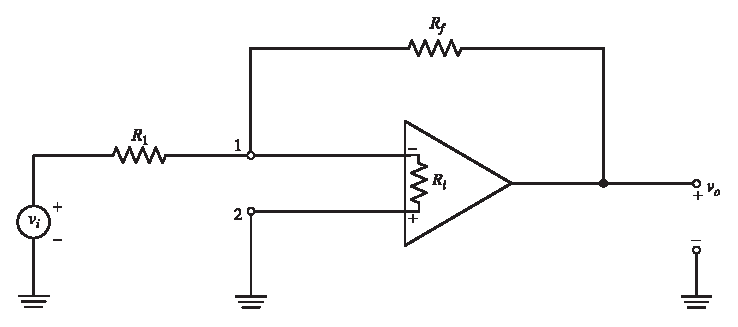
\includegraphics{chap4/S3-EE-06-018.eps}
\smallskip
\caption{Op-amp inverting amplifier}\label{fig5.11}
\end{figure}

\vfill\eject

Due to virtual short at the input of Op-amp, terminals 1 \&\ 2 appear to be tied together. Fig.~\ref{fig5.12} shows the equivalent circuit at the input side.
\begin{figure}[H]
\centering
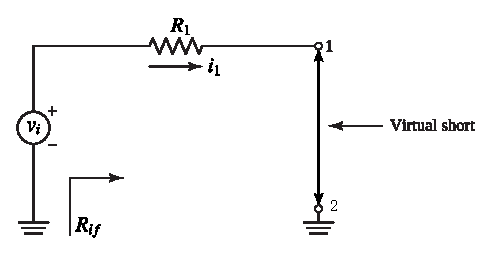
\includegraphics{chap4/S3-EE-06-019.eps}
\smallskip
\caption{Circuit to find input resistance}\label{fig5.12}
\end{figure}

Input resistance $R_{if}$ of the amplifier with negative feedback is nothing but the resistance seen by the input signal $v_{i}$
\begin{equation}
\therefore\quad R_{if}=\frac{v_{i}}{i_{1}}\label{eq5.28}
\end{equation}
but for the circuit of Fig.~\ref{fig5.12}.
\begin{align}
v_{i} &= i_{1}R_{1}\notag\\[3pt]
\Rightarrow\quad \frac{v_{i}}{i_{1}} &= R_{1}\label{eq5.29}
\end{align}

Combining Eqns.~\eqref{eq5.28} and \eqref{eq5.29} we have
\begin{equation}
R_{if}=R_{1}\label{eq5.30}
\end{equation}

\begin{example}\label{exam5.16}
Design an Op-amp inverting amplifier with a gain of $-50$ and a $2\,k\Omega$ input resistance.
\end{example}

\begin{solution}
\vskip -.6cm
\begin{align*}
A_{f} &= -50, \ R_{if}=2 k\Omega\\[2pt]
R_{1} &= R_{if}=2 k\Omega\\[2pt]
A_{f} &= \frac{-R_{f}}{R_{1}}=-50\\[2pt]
R_{f} &= 50 R_{1}\\[2pt]
&= 50 \times 2 k\Omega\\[2pt]
&= 100 k\Omega
\end{align*}
The inverting amplifier circuit is shown below
\begin{figure}[H]
\centering
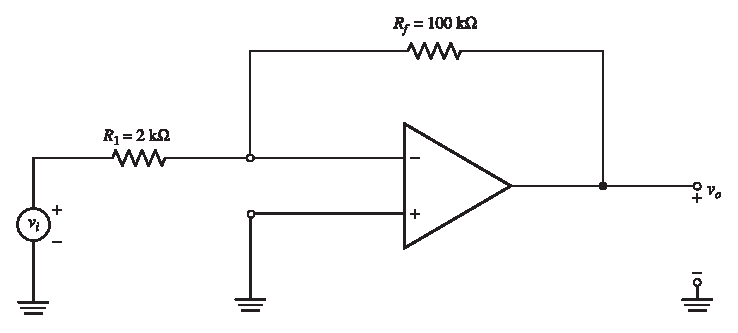
\includegraphics{chap4/S3-EE-06-IN009.eps}
\end{figure}
\end{solution}

\begin{example}\label{exam5.17}
For the circuit shown below, find
\begin{itemize}
\item[(i)] Closed loop voltage gain, $A_{f}$.

\item[(ii)] Input resistance, $R_{if}$.

\item[(iii)] Current flowing through $R_{1}$ if $v_{i}=0.5\,$V.
\end{itemize}
\begin{figure}[H]
\centering
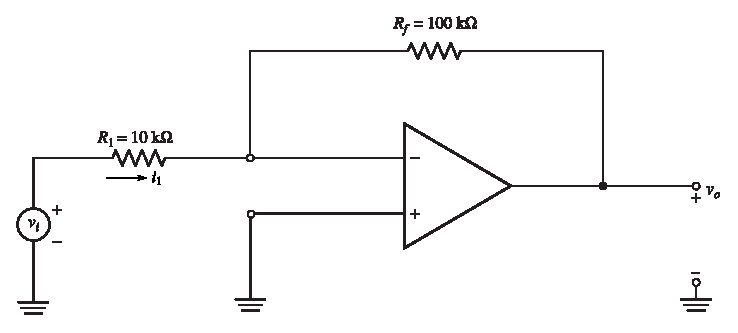
\includegraphics{chap4/S3-EE-06-IN010.eps}
\end{figure}
\end{example}

\begin{solution}
~

\begin{itemize}
\item[(i)] 
\begin{tabbing}
$A_{f}$ \== $\dfrac{-R_{f}}{R_{1}}= \dfrac{-100\,k\Omega}{10\,k\Omega}$\\[4pt]
\>= $-10$
\end{tabbing}

\item[(ii)] $R_{if}=R_{1}=10 k\Omega$

\item[(iii)] Current through $R_{1}$ is
\begin{align*}
i_{1} &= \frac{v_{i}}{R_{1}}= \frac{0.5\,\text{V}}{10\,k\Omega}\\[3pt]
&= 0.05\text{\, mA~~ or~~ } 50\mu \text{\,A}
\end{align*}
\end{itemize}
\vskip -1.05cm
\end{solution}

\section{Linear Applications of Op-amp}\label{addsec5.12}
\index{Applications of Op-amp}

When an Op-amp is used for linear applications, the output and input voltages are related by a linear function. Some of the linear applications of\index{Operational amplifier!applications of} Op-amp are as follows.
\begin{enumerate}
\itemsep=1pt
\item Voltage follower

\item Adder or summing amplifier 

\item Subtractor

\item Integrator

\item Differentiator
\end{enumerate}

\section{Voltage follower}\label{sec5.11}

A voltage follower is a circuit in which the output voltage $v_{o}$ follows the input voltage $v_{i}$. Note that the voltage gain of voltage follower\index{Voltage follower}\index{Operational amplifier!voltage follower}\index{Applications of Op-amp!voltage follower} is unity, since $v_{o}=v_{i}$.

The circuit of voltage follower can be derived from the non-inverting amplifier by short circuiting $R_{f}$ and open circuiting $R_{1}$ i.e. by setting $R_{f}=0$ and $R_{1}=\infty$. Fig.~\ref{fig5.13} shows the circuit of an Op-amp voltage follower.

Since the input voltage $v_{i}$ is directly applied to the non-inverting input terminals
\begin{equation}
v_{2}=v_{i}\label{eq5.31}
\end{equation}

Due to virtual short at the input of Op-amp, the inverting and non-inverting input terminals are at the same potential
\begin{equation}
\therefore\quad v_{1}=v_{2}\label{eq5.32}
\end{equation}

Also note that the inverting input terminal is directly tied to the output terminal
\begin{equation}
\therefore\quad v_{o}=v_{1}\label{eq5.33}
\end{equation}

\begin{figure}[H]
\centering
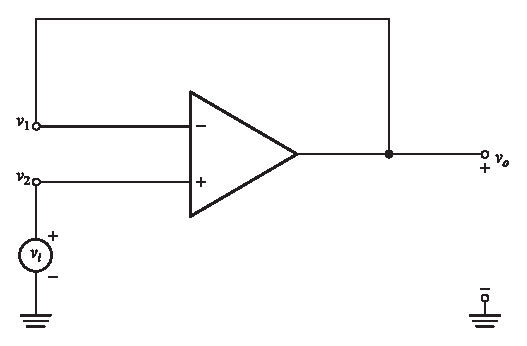
\includegraphics{chap4/S3-EE-06-021.eps}
\caption{Op-amp voltage follower}\label{fig5.13}
\end{figure}

Combining Eqns.~\eqref{eq5.31}, \eqref{eq5.32} and \eqref{eq5.33} we have
\begin{equation}
v_{o}=v_{i}\label{eq5.34}
\end{equation}

From Eqn.~\eqref{eq5.34} we find that output voltage follows the input voltage. The closed loop voltage gain is given by
\begin{equation}
A_{f}=\frac{v_{o}}{v_{i}}=1\label{eq5.35}
\end{equation}
Note that the closed loop voltage gain is unity.

\section{Important properties of Op-amp voltage follower}\label{sec5.12}

The important properties of\index{Voltage follower!properties of} an Op-amp voltage follower are listed below:
\begin{itemize}
\item[(i)] Extremely high input resistance.

\item[(ii)] Very low output resistance.

\item[(iii)] Large bandwidth.

\item[(iv)] Unity voltage gain due to 100\% negative feed back.
\end{itemize}

\heading{Application of\index{Voltage follower!application of} voltage follower}

Voltage follower is used as buffer to feed a low resistance load from a voltage source of high source resistance.

\noindent
{\bf Note:}~The feedback factor in Op-amp non-inverting amplifier is given by
\begin{align*}
\beta &= \frac{R_{1}}{R_{1}+R_{f}}=\frac{1}{1+\left(\frac{R_{f}}{R_{1}}\right)}\\
\text{with}\quad R_{f} &=0 \text{~~ and~~ } R_{1}=100,\text{~~ we get}\\
\beta &= 1\Rightarrow 100\%\text{~~ negative feed back.}
\end{align*}

\section{Op-amp summer or summing amplifier}\label{sec5.13}
\index{Summing amplifier}

Fig.~\ref{fig5.14} shows the circuit of an Op-amp summer.\index{Operational amplifier!summer}\index{Applications of Op-amp!summer}
\begin{figure}[H]
\centering
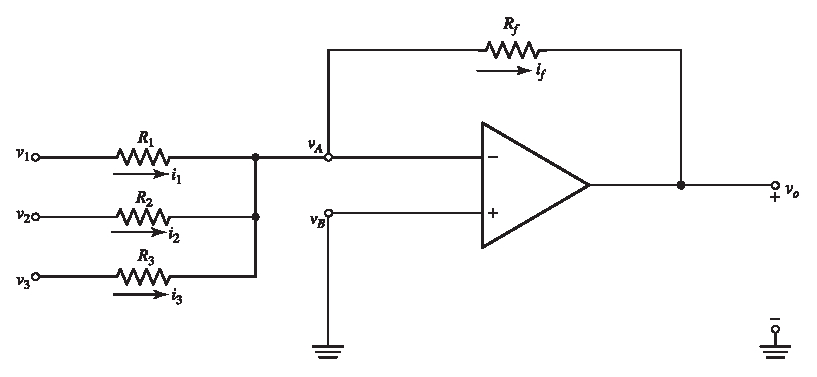
\includegraphics{chap4/S3-EE-06-023.eps}
\caption{Op-amp Summer}\label{fig5.14}
\end{figure}

Since the non-inverting input terminal of Op-amp is grounded $v_{B}=0$. Due to virtual short at the input of Op-amp, the inverting and non-inverting input terminals are at the same potential.
\begin{align}
\therefore\quad v_{A} &= v_{B}=0\notag\\
i_{1} &= \frac{v_{1}-v_{A}}{R_{1}}=\frac{v_{1}}{R_{1}}\label{eq5.36}\\
i_{2} &= \frac{v_{2}-v_{A}}{R_{2}}=\frac{v_{2}}{R_{2}}\label{eq5.37}\\
i_{3} &= \frac{v_{3}-v_{A}}{R_{3}}=\frac{v_{3}}{R_{3}}\label{eq5.38}\\
i_{f} &= \frac{v_{A}-v_{o}}{R_{f}}=\frac{-v_{o}}{R_{f}}\label{eq5.39}
\end{align}

Due to high input impedance of the Op-amp, the current flowing into its inverting input terminal is zero. Applying Kirchhoff's Current Law at the node $v_{A}$ we have
\begin{equation}
i_{f}=i_{i}+i_{2}+i_{3}\label{eq5.40}
\end{equation}

Substituting for $i_{1}$, $i_{2}$, $i_{3}$ and $i_{f}$ we have
\begin{align}
\frac{-v_{o}}{R_{f}} &= \frac{v_{1}}{R_{1}}+\frac{v_{2}}{R_{2}}+\frac{v_{3}}{R_{3}}\notag\\[4pt]
v_{o} &= -\left[\frac{R_{f}}{R_{1}}v_{1}+\frac{R_{f}}{R_{2}}v_{2}+\frac{R_{f}}{R_{3}}v_{3}\right]\label{eq5.40}
\end{align}

If we choose $R_{f}=R_{1}=R_{2}=R_{3}$, then
\begin{equation}
v_{0}=-[v_{1}+v_{2}+v_{3}]\label{eq5.42}
\end{equation}
Note that the output voltage is equal to the negative of the sum of the input voltages. The circuit is called inverting summer due to the negative sign.

\begin{example}\label{exam5.18}
For the circuit shown below calculate the output voltage
\begin{figure}[H]
\centering
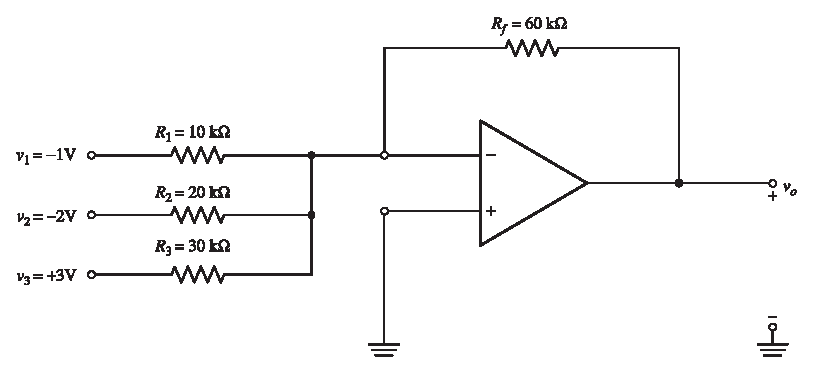
\includegraphics{chap4/S3-EE-06-IN011.eps}
\end{figure}
\end{example}

\begin{solution}
\begin{align*}
v_{o} &= -\left[\frac{R_{f}}{R_{1}}v_{1}+\frac{R_{f}}{R_{2}}v_{2}+\frac{R_{f}}{R_{3}}v_{3}\right]\\[4pt]
&= -\left[\frac{60\, k\Omega}{10\, k\Omega}(-1\text{\,V})+\frac{60\, k\Omega}{20\, k\Omega}(-2\text{\,V})+\frac{60\, k\Omega}{30\, k\Omega}(3\text{\,V})\right]\\[4pt]
&= - [-6\text{\,V}-6\text{\,V}+6\text{\,V}]=6\text{\,V}
\end{align*}
\vskip -1cm
\end{solution}

\eject

\begin{example}\label{exam5.19}
Calculate the output voltage of a three-input summing amplifier given that
\begin{alignat*}{2}
& R_{1}=200\, k\Omega &\qquad& v_{1}=-2V\\
& R_{2}=250\, k\Omega &\qquad& v_{2}=2V\\
& R_{3}=500\, k\Omega &\qquad& v_{3}=1V\\
& R_{f}=1 M\Omega &&
\end{alignat*}
\end{example}

\begin{solution}
\begin{align*}
v_{o} &= - \left[\frac{R_{f}}{R_{1}}v_{1}+\frac{R_{f}}{R_{2}}v_{2}+\frac{R_{f}}{R_{3}}v_{3}\right]\\[4pt]
&= -\left[\frac{10^{6}\Omega}{200\times 10^{3}\Omega}(-2V)+\frac{10^{6}\Omega}{250\times 10^{3}\Omega}(2V)+\frac{10^{6}\Omega}{500\times 10^{3}\Omega}(1V)\right]\\[4pt]
&= -[-10V+8V+2V]\\[4pt]
&= 0V
\end{align*}
\vskip -.7cm
\end{solution}

\begin{example}\label{exam5.20}
For the circuit shown determine the output voltage.
\begin{figure}[H]
\centering
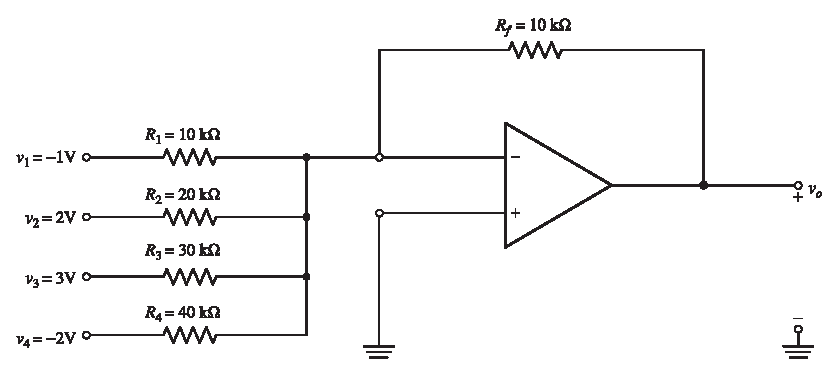
\includegraphics{chap4/S3-EE-06-IN012.eps}
\end{figure}
\end{example}

\begin{solution}
\begin{align*}
v_{o} &= -\left[\frac{R_{f}}{R_{1}}v_{1}+\frac{R_{f}}{R_{2}}v_{2}+\frac{R_{f}}{R_{3}}v_{3}+\frac{R_{f}}{R_{4}}v_{4}\right]\\[4pt]
&= -\left[\frac{10\, k\Omega}{10\, k\Omega}(-1V)+\frac{10\, k\Omega}{20\, k\Omega}(2V)+\frac{10\, k\Omega}{30\, k\Omega}(3V)+\frac{10\, k\Omega}{40\, k\Omega}(-2)\right]\\[4pt]
&= +\,0.5 V
\end{align*}
\vskip -.7cm
\end{solution}

\eject

\begin{example}\label{exam5.21}
Design an adder circuit using Op-amp to obtain an output voltage given by
$$
v_{1}=-[0.5v_{1}+0.8v_{2}+2v_{3}]
$$
where $v_{1}$, $v_{2}$ and $v_{3}$ are the inputs.
\end{example}

\begin{solution}
Given,
\begin{equation*}
v_{o}=-[0.5v_{1}+0.8v_{2}+2v_{3}]\tag{A}
\end{equation*}
The output voltage of an Op-amp adder is given by
\begin{equation*}
v_{o}=-\left[\frac{R_{f}}{R_{1}}v_{1}+\frac{R_{f}}{R_{2}}v_{2}+\frac{R_{f}}{R_{3}}v_{3}\right]\tag{B}
\end{equation*}
Comparing Eqns.~(A) and (B) we have
\begin{align*}
\frac{R_{f}}{R_{1}} &= 0.5\Rightarrow R_{1}=2R_{f}\\[3pt]
\frac{R_{f}}{R_{2}} &= 0.8\Rightarrow R_{2}=1.25 R_{f}\\[3pt]
\frac{R_{f}}{R_{3}} &= 2 \Rightarrow R_{3}=0.5 R_{f}
\end{align*}
Select $R_{f}=10 k\Omega$.
\begin{align*}
\therefore\quad R_{1} &= 2\times 10\, k\Omega = 20\,k\Omega\\[3pt]
R_{2} &= 1.25 \times 10\,k\Omega = 12.5\,k\Omega\\[3pt]
R_{3} &= 0.5 \times 10\,k\Omega = 5\,k\Omega
\end{align*}
The adder circuit with component values is shown below.
\begin{figure}[H]
\centering
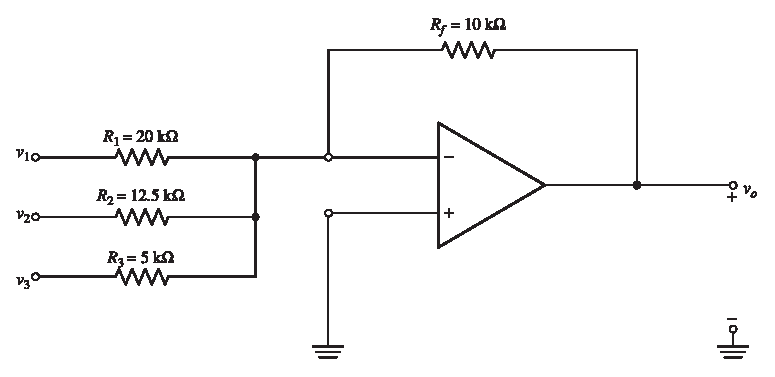
\includegraphics{chap4/S3-EE-06-IN013.eps}
\end{figure}
\vskip -1cm
\end{solution}

\eject

\begin{example}\label{exam5.22}
Design an adder circuit using Op-amp to obtain an output voltage given by, $v_{o}=2[0.1 v_{1}+0.5v_{2}+2.0\,v_{3}]$ where $v_{1}$, $v_{2}$ and $v_{3}$ are the input voltages.
\end{example}

\begin{solution}
Given,
\begin{align*}
v_{0} &= 2[0.1v_{1}+0.5v_{2}+2v_{3}]\\[3pt]
      &= [0.2v_{1}+v_{2}+4v_{3}]\\[3pt]
      &= -[0.2v_{1}+v_{2}+4v_{3}][-1]\\[3pt] 
      &= v'_{0}[-1]\tag{A}\\[3pt]
\text{where,}\quad v'_{0} &= -[0.2v_{1}+v_{2}+4v_{3}]\tag{B}
\end{align*}
The output voltage of an Op-amp adder is given by
\begin{equation*}
v'_{0} =-\left[\frac{R_{f}}{R_{1}}v_{1}+\frac{R_{f}}{R_{2}}v_{2}+\frac{R_{f}}{R_{3}}v_{3}\right]\tag{C}
\end{equation*}
Comparing Eqns.~(B) and (C) we have
\begin{align*}
\frac{R_{f}}{R_{1}} &= 0.2\Rightarrow R_{1}=5R_{f}\\[5pt]
\frac{R_{f}}{R_{2}} &= 1 \Rightarrow R_{2}=R_{f}\\[5pt]
\frac{R_{f}}{R_{3}} &= 4 \Rightarrow R_{3}=0.25 R_{f}
\end{align*}
Select~ $R_{f}=10 k\Omega$.
\begin{align*}
\text{Now,}\qquad R_{1} &= 5\times 10\, k\Omega=50\, k\Omega\\[5pt]
R_{2} &= 10\, k\Omega\\[5pt]
R_{3} &= 0.25\times 10\, k\Omega= 2.5\, k\Omega
\end{align*}

The summer output is $v'_{0}$. To obtain, $v_{0}=-v'_{0}$, $v_{0}$ should be applied to an inverting amplifier of gain $-1$. The required circuit is shown below.
\begin{figure}[H]
\centering
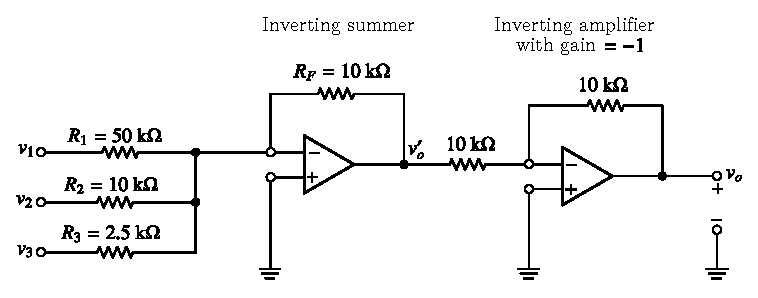
\includegraphics{chap4/S3-EE-06-IN014.eps}
\end{figure}
\vskip -.7cm
\end{solution}

\begin{example}\label{exam5.23}
Design an Op-amp circuit so that the output $v_{0}=0.8v_{1}+0.6v_{2}-2v_{3}$ is realised.
\end{example}

\begin{solution}
Given,
\begin{align*}
v_{0} &= 0.8v_{1}+0.6v_{2}-2v_{3}\\[3pt]
     &= -[-0.8v_{1}-0.6v_{2}]-2v_{3}\\[3pt]
     &= -v'-2v_{3}\\[3pt]
\text{or}\qquad v_{0} &=-[v'+2v_{3}]\tag{A}\\[4pt]
\text{where}\qquad v' &= -0.8v_{1}-0.6v_{2}\\[3pt]
\text{or}\qquad v' &= -[0.8v_{1}+0.6v_{2}]\tag{B}
\end{align*}

First we realise Eqn.~(B) and obtain $v'$. Then Eqn.~(A) is realised. We need two inverting summers.

\medskip

\heading{To obtain \boldmath$v'$}

From Eqn.~(B)
$$
\dfrac{R_{f}}{R_{1}}=0.8\quad\Rightarrow\quad R_{1}=1.25\,R_{f}
$$
and
$$
\dfrac{R_{f}}{R_{2}}=0.6\quad\Rightarrow\quad R_{2}=1.67\,R_{f}
$$
we choose, $R_{f}=10\,k\Omega$
\begin{align*}
\therefore\qquad R_{1} &= 1.25\times 10\,k\Omega=12.5\,k\Omega\\[3pt]
\text{and}\qquad R_{2} &= 1.67\times 10\,k\Omega=16.7\,k\Omega
\end{align*}

\eject

\heading{To obtain \boldmath$v_{0}$}

From Eqn.~(A)
\begin{align*}
& \dfrac{R'_{f}}{R'_{1}}=1\quad\Rightarrow\quad R'_{f}=R'_{1}\\[3pt]
\text{and}\qquad & \frac{R'_{f}}{R'_{2}}=2\quad\Rightarrow\quad R'_{2}=0.5R'_{f}
\end{align*}
If we choose, $R'_{f}=10\,k\Omega$, then
$$
R'_{1}=10\,k\Omega\quad\text{and}\quad R'_{2}=5\,k\Omega
$$
The required circuit is shown below.
\begin{figure}[H]
\centering
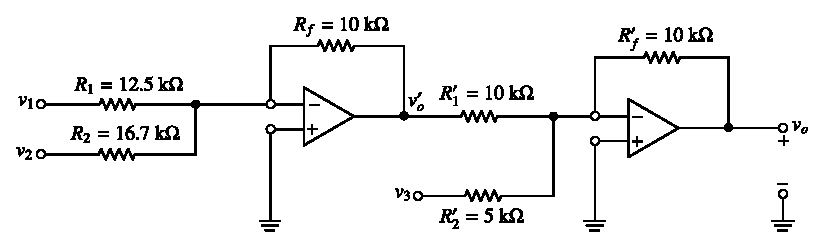
\includegraphics{chap4/S3-EE-06-IN015.eps}
\end{figure}
\vskip -1cm
\end{solution}

\section{Op-amp subtractor}\label{sec5.15}
\index{Op-amp subtractor}

Fig.~5.16(a) shows the circuit of an Op-amp subtractor.\index{Operational amplifier!subtractor}\index{Applications of Op-amp!subtractor}
\begin{figure}[H]
\centering
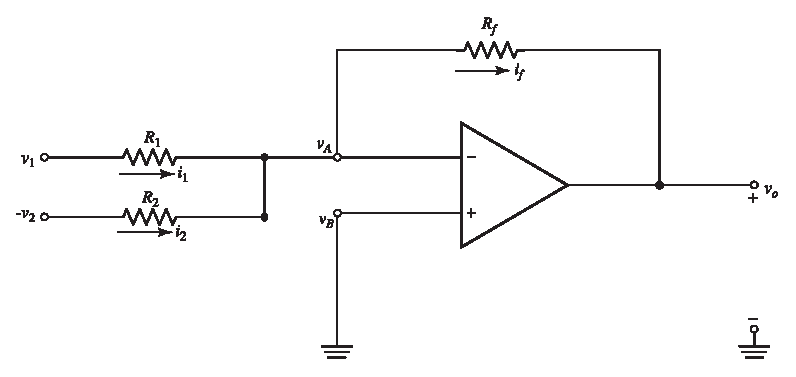
\includegraphics{chap4/S3-EE-06-024.eps}

\medskip
\centerline{\colorbox{lightgray}{~~~{\bf Fig.\,5.16(a):~}{\em Op-amp subtractor}~~~}}
\end{figure}

\eject

Since the non-inverting input terminal of Op-amp is grounded, $v_{B}=0$. Due to virtual short at the input of Op-amp, the inverting and non-inverting input terminals are at the same potential.
\begin{align}
\therefore\quad v_{A} &= v_{B}=0\notag\\
i_{1} &= \frac{v_{1}-v_{A}}{R_{1}}=\frac{v_{1}}{R_{1}}\label{eq5.43}\\
i_{2} &= \frac{(-v_{2})-v_{A}}{R_{2}}=\frac{-v_{2}}{R_{2}}\label{eq5.44}\\
i_{f} &= \frac{v_{A}-v_{o}}{R_{f}}=\frac{-v_{o}}{R_{f}}\label{eq5.45}
\end{align}


Due to high input impedance of Op-amp, the current flowing into its inverting input terminal is zero. Applying Kirchhoff's Current Law at the node $v_{A}$ we have
\begin{equation}
i_{f}=i_{1}+i_{2}\label{eq5.46}
\end{equation}
substituting for $i_{1}$, $i_{2}$ and $i_{f}$ we have
\begin{align*}
\frac{-v_{o}}{R_{f}} &= \frac{v_{1}}{R_{1}}-\frac{v_{2}}{R_{2}}\\
v_{o} &= -\frac{R_{f}}{R_{1}}v_{1}+\frac{R_{f}}{R_{2}}v_{2}
\end{align*}
If we select $R_{f}=R_{1}=R_{2}=R$, then
\begin{equation}
v_{o}=(v_{2}-v_{1})\label{eq5.47}
\end{equation}
Eqn.~\eqref{eq5.47} shows that the output is the difference of the two inputs. Therefore an Op-amp can be used as a subtractor.

The voltage, $-v_{2}$ can be obtained from $v_{2}$ using an inverting amplifier of gain, $-1$, as shown in Fig.~5.16(b).
\begin{figure}[H]
\centering
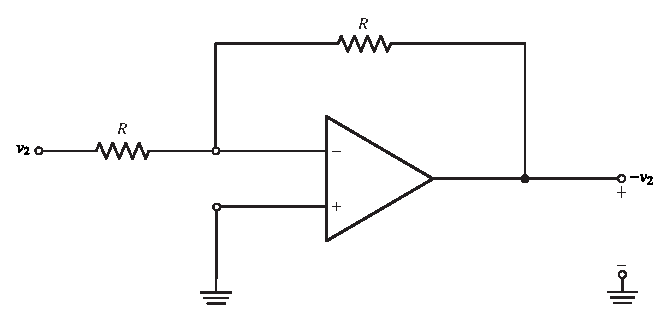
\includegraphics{chap4/fig4.14b.eps}

\medskip
\centerline{\colorbox{lightgray}{{\bf Fig.\,5.16(b):~}{\em Inverting amplifier with gain, $-1$}}}
\end{figure}

The complete circuit of subtractor is shown in Fig.~5.16(c).
\begin{figure}[H]
\centering
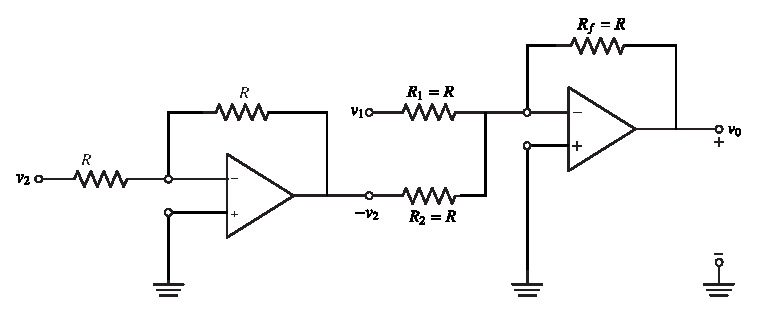
\includegraphics{chap4/fig4.14c.eps}

\medskip
\centerline{\colorbox{lightgray}{~~~{\bf Fig.\,5.16(c):~}{\em Complete circuit of subtractor}~~~}}
\end{figure}

\section{Alternate circuit for subtractor}\label{sec5.15}

Fig.~\ref{fig5.16} shows an alternate circuit of Op-amp subtractor.\index{Op-amp subtractor}
\setcounter{figure}{16}
\begin{figure}[H]
\centering
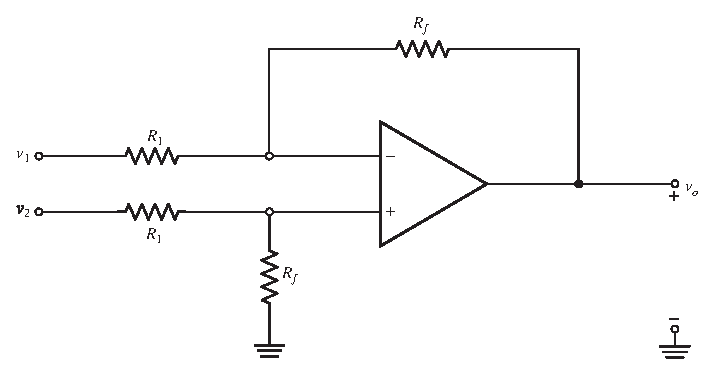
\includegraphics{chap4/fig4.15.eps}
\caption{Alternate circuit for subtractor}\label{fig5.16}
\end{figure}

Let us obtain the output voltage $v_{o}$ using superposition principle by applying the following steps.

\eject

\begin{description}
\item[{\bf Step 1:}] Reduce $v_{2}$ to zero and find the output voltage $v_{o1}$ due to $v_{1}$. The resulting circuit is shown in Fig.~\ref{fig5.17} which is nothing but an inverting amplifier.
\begin{figure}[H]
\centering
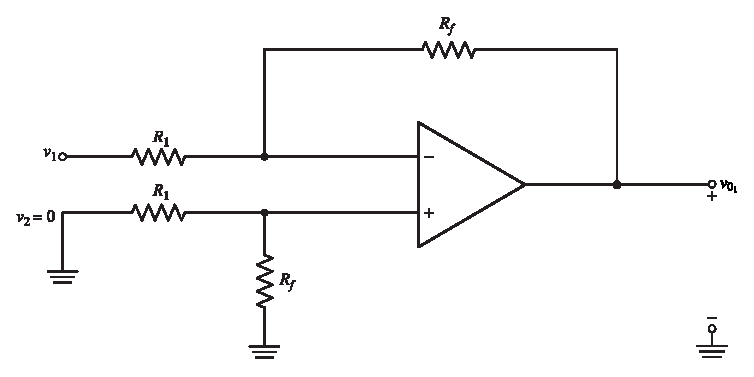
\includegraphics{chap4/S3-EE-06-025.eps}
\caption{Circuit to find output voltage $v_{01}$ due to $v_{1}$}\label{fig5.17}
\end{figure}
\begin{equation}
v_{o_{1}}=-\left[\frac{R_{f}}{R_{1}}\right]v_{1}\label{eq5.48}
\end{equation}

\item[{\bf Step 2:}] Reduce $v_{1}$ to zero and find the output voltage $v_{o2}$ due to $v_{2}$. The resulting circuit is shown in Fig.~\ref{fig5.18} which is nothing but a non-inverting amplifier.
\begin{figure}[H]
\centering
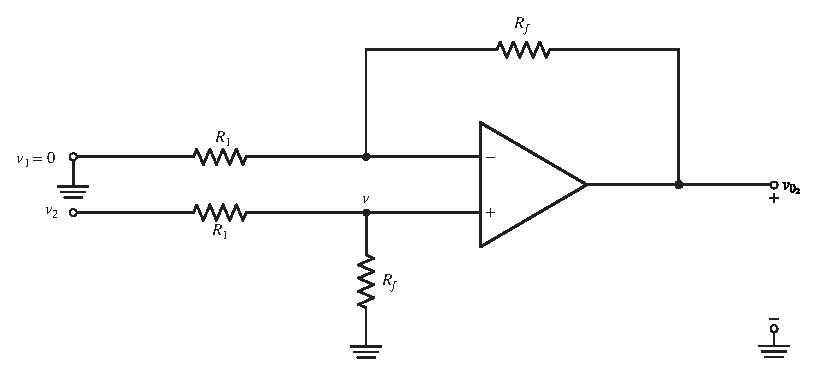
\includegraphics{chap4/S3-EE-06-026.eps}
\caption{Circuit to find output voltage $v_{02}$ due to $v_{2}$}\label{fig5.18}
\end{figure}

\eject

~\phantom{a}

\vskip -1.3cm

\begin{align}
v_{o_{2}} &= v\times \text{~Gain of non-inverting amplifier}\notag\\[4pt]
       &= v\left[1+\frac{R_{f}}{R_{1}}\right]\label{eq5.49}
\end{align}
$v$ is the voltage drop across $R_{f}$. Using voltage division rule
\begin{align}
v &= v_{2}\left[\frac{R_{f}}{R_{1}+R_{f}}\right]\notag\\[5pt]
  &= v_{2}\frac{R_{f}}{R_{1}[1+R_{f}/R_{1}]}\label{eq5.50} 
\end{align}
Substituting Eqn.~\eqref{eq5.50} into Eqn.~\eqref{eq5.49}, we have
\begin{align}
v_{o_{2}} &= v_{2}\,\frac{R_{f}}{R_{1}[1+R_{f}/R_{1}]}\,[1+R_{f}/R_{1}]\notag\\[7pt]
       &= v_{2}\,[R_{f}/R_{1}]\label{eq5.51}
\end{align}

\item[{\bf Step 3:}] Resultant output voltage is given by the superposition principle
\begin{align}
v_{o} &= v_{o_{1}}+v_{o_{2}}\notag\\[7pt]
&= -\frac{R_{f}}{R_{1}}v_{1}+\frac{R_{f}}{R_{1}}v_{2}\notag\\[7pt]
v_{o}&= \frac{R_{f}}{R_{1}}[v_{2}-v_{1}]\label{eq5.52}
\end{align}
If we choose $R_{f}=R_{1}$, then
\begin{equation}
v_{o}=[v_{2}-v_{1}]\label{eq5.53}
\end{equation}
From Eqn.~\eqref{eq5.53} we find that the output voltage is the difference of the two input voltages. Hence the given circuit works as subtractor.
\end{description}

\eject

\section{Op-amp as an integrator}\label{sec5.16}
\index{Operational amplifier!integrator}\index{Applications of Op-amp!integrator}

Fig.~\ref{fig5.19} shows an Op-amp integrator.\index{Op-amp integrator} It has a capacitor in the feedback loop.
\begin{figure}[H]
\centering
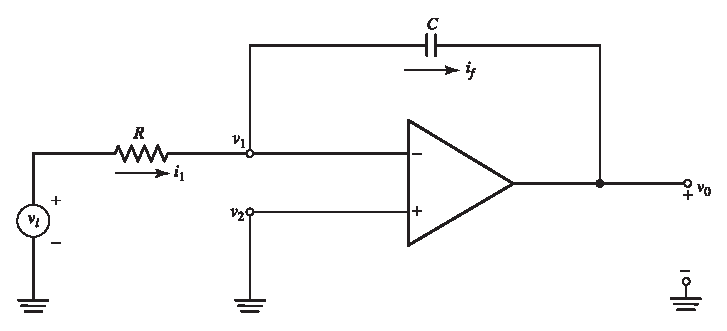
\includegraphics{chap4/S3-EE-06-027.eps}
\caption{Op-amp integrator}\label{fig5.19}
\end{figure}

Since the non-inverting input terminal of Op-amp is grounded, $v_{2}=0$. Due to virtual short at the input of Op-amp, the inverting and non-inverting input terminals are at the same potential.
$$
\therefore\quad v_{1}=v_{2}=0
$$
Due to high input impedance of Op-amp, the current flowing into its inverting input terminal is zero. Therefore same current flows through $R$ and $C$
\begin{equation}
\text{i.e.,}\quad i_{1}=i_{f}\label{eq5.54}
\end{equation}
But
\begin{equation}
i_{1}=\frac{v_{i}-v_{1}}{R}=\frac{v_{i}}{R}\label{eq5.55}
\end{equation}
and
\begin{equation}
i_{f}=C\,\frac{d}{dt}[v_{1}-v_{o}]=-C\,\dfrac{dv_{o}}{dt}\label{eq5.56}
\end{equation}
Substituting these relations in Eqn.~\eqref{eq5.54} we have
\begin{align*}
\frac{v_{i}}{R} &=-C\,\frac{dv_{o}}{dt}\\[3pt]
\frac{dv_{o}}{dt} &= -\frac{1}{RC}\,v_{i}
\end{align*}
Integrating both sides with respect to `$t$' we have
\begin{equation}
v_{o}=-\frac{1}{RC}\int\limits^{t}_{0}v_{i}\,dt+v_{o}(0)\label{eq5.57}
\end{equation}
where $v_{o}(0)$ is the initial voltage on the capacitor at $t=0$. Note that $v_{o}(0)$ represents the constant of integration. From Eqn.~\eqref{eq5.57} we find that the output voltage $v_{o}$ is proportional to the integral of the input voltage $v_{i}$.

If the initial voltage on the capacitor at $t=0$ is zero then, $v_{o}(0)=0$. Now Eqn.~\eqref{eq5.57} can be written as
\begin{equation}
v_{o}=-\frac{1}{RC}\int\limits^{t}_{0}v_{i}\,dt\label{eq5.58}
\end{equation}

\section{Op-amp as differentiator}\label{sec5.17}

Fig.~\ref{fig5.20} shows an Op-amp differentiator.\index{Op-amp differentiator} The circuit of Op-amp differentiator\index{Operational amplifier!differentiator}\index{Applications of Op-amp!differentiator} can be obtained from Op-amp integrator circuit by simply interchanging the positions of $R$ and $C$.
\begin{figure}[H]
\centering
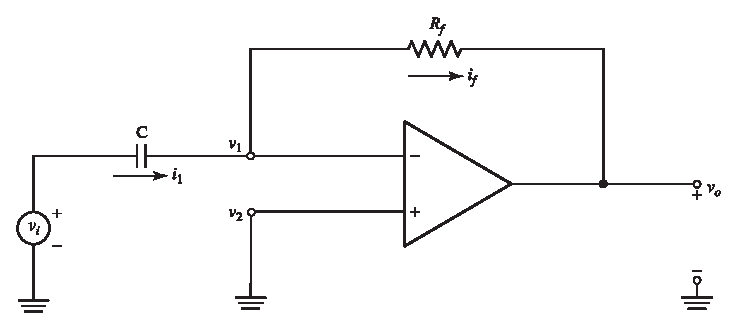
\includegraphics{chap4/S3-EE-06-028.eps}
\caption{Op-amp differentiator}\label{fig5.20}
\end{figure}

Since the non-inverting input terminal of Op-amp is grounded $v_{2}=0$. Due to virtual short at the input of Op-amp, the inverting and non-inverting input terminals are at the same potential.
$$
\therefore\quad v_{1}=v_{2}=0.
$$

Due to high input impedance of Op-amp, the current flowing into its inverting input terminal is zero. Therefore, same current flows through $R$ and $C$
\begin{equation}
\text{i.e.,}\quad i_{1}=i_{f}\label{eq5.59}
\end{equation}

But
\begin{equation}
i_{1}=C\,\frac{d}{dt}[v_{i}-v_{1}]=C\,\frac{dv_{i}}{d_{t}}\label{eq5.60}
\end{equation}
and
\begin{equation}
i_{f}=\frac{v_{i}-v_{o}}{R}=\frac{-v_{o}}{R}\label{eq5.61}
\end{equation}

Using these relations in Eqn.~\eqref{eq5.59} we have
\begin{align}
C\,\dfrac{dv_{i}}{dt} &= -\,\frac{v_{o}}{R}\notag\\[3pt]
v_{o} &= -RC\;\frac{dv_{i}}{dt}\label{eq5.62}
\end{align}
Eqn.~\eqref{eq5.62} shows that the output voltage $v_{o}$ is proportional to the time derivative of the input voltage $v_{i}$.

\begin{example}\label{exam5.25}
The integrator circuit of Fig.~\ref{fig5.19} has $R=500\,k\Omega$ and $C=1\,\mu F$. Find and plot the output voltage for the inputs given below
\begin{center}
\begin{tabular}{r@{\;\;}l@{\qquad\qquad\qquad}r@{\;\;}l}
(a) & \raisebox{-1cm}{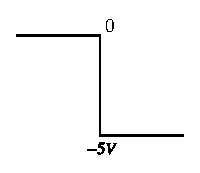
\includegraphics{chap4/exp4.25a.eps}} & (b) & \raisebox{-1cm}{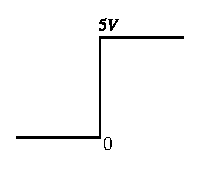
\includegraphics{chap4/exp4.25b.eps}}\\[40pt]
(c) & $v_{i}=2\sin 4t\text{V}$ & (d) & $v_{i}=4t\text{\,V}$
\end{tabular}
\end{center}
Assume that, the initial voltage on capacitor is zero.
\end{example}

\begin{solution}
\begin{equation*}
v_{0}=-\frac{1}{RC}\int\limits^{t}_{0}v_{i}dt+v_{0}(0)\tag{A}
\end{equation*}
Given, \ $R=500\,k\Omega$, $C=1\mu F\Rightarrow \dfrac{1}{RC}=2$ \ and \ $v_{0}(0)=0$.

To obtain $v_{0}$ as a function of `$t$', we integrate with out limits.
\begin{equation*}
\therefore\qquad v_{0}=-2\int v_{i}dt\tag{B}
\end{equation*}
\begin{itemize}
\item[(a)] 
\begin{tabular}[t]{c@{\hspace{3.07cm}}c}
\begin{tabular}[t]{@{}l}
$v_{i}= -5\text{V}(DC)$\\[3pt]
$v_{0}= -2\int (-5) dt = +10\,t\text{V}$
\end{tabular}&
\raisebox{-1.4cm}{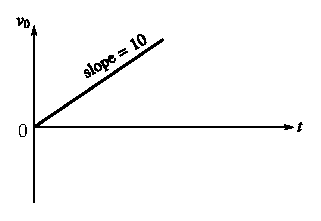
\includegraphics{chap4/sol4.25a.eps}}
\end{tabular}

~

\item[(b)]
\begin{tabular}[t]{c@{\hspace{3.25cm}}c}
\begin{tabular}[t]{@{}l}
$v_{i}= 5\text{V}(DC)$\\[3pt]
$v_{0}= -2\int 5dt = -10\,t\text{V}$
\end{tabular}&
\raisebox{-1.4cm}{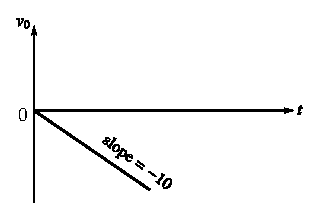
\includegraphics{chap4/sol4.25b.eps}}
\end{tabular}

~ 

\item[(c)]
\begin{tabular}[t]{c@{\hspace{3.6cm}}c}
\begin{tabular}[t]{@{}r@{\;}l}
$v_{i}\,$ & $= 2\sin 4t\,\text{V}$\\[3pt]
$v_{0}$   & $= -2\int 2 \sin 4t\,dt$\\[3pt]
          & $= -4\left[\dfrac{-\cos 4t}{4}\right]$\\[3pt]
         &  $= \cos 4\,t\,\text{V}$
\end{tabular}&
\raisebox{-2.7cm}{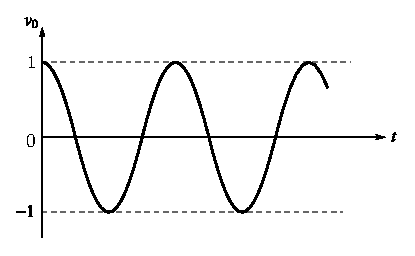
\includegraphics{chap4/sol4.25c.eps}}
\end{tabular}

~

\item[(d)]
\begin{tabular}[t]{c@{\hspace{4.5cm}}c}
\begin{tabular}[t]{@{}r@{\;}l}
$v_{i}\,$ & $= 4\,t\,\text{V}$\\[3pt]
$v_{0}$   & $= -2\int 4t\, dt$\\[3pt]
          & $= -8[t^{2}/2]$\\[3pt]
          & $= -4\,t^{2}\,\text{V}$
\end{tabular}&
\raisebox{-2.2cm}{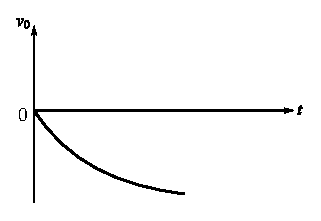
\includegraphics{chap4/sol4.25d.eps}}
\end{tabular}
\end{itemize}
\end{solution}

\begin{example}\label{exam5.26}
The differentiator circuit of Fig.~\ref{fig5.20} has $R=1 M\Omega$ and $C=1\mu F$. Find and plot the output voltages for the following inputs.
\begin{center}
\begin{tabular}{r@{\;}l@{\qquad}r@{\;}l@{\qquad}r@{\;}l@{\qquad}r@{\;}l}
(a) & $v_{i}=10\,t\,\text{V}$ & (b) & $v_{i}=-5\,t\,\text{V}$ &
(c) & $v_{i}=2\,t^{2}\,\text{V}$ & (d) & $v_{i}=2\cos 2\,t\,\text{V}$
\end{tabular}
\end{center}
\end{example}

\eject

\begin{solution}
Given,
\begin{align*}
R &= 1 M\Omega\quad C=1\mu F\Rightarrow RC=1\\[3pt]
v_{0} &=-\, RC\,\dfrac{dv_{i}}{dt}
\end{align*}
Substituting the value of $RC$, we get
$$
v_{0}=-\dfrac{dv_{i}}{dt}
$$
\smallskip
\begin{itemize}
\item[(a)]
\begin{tabular}[t]{c@{\hspace{3.2cm}}c}
\begin{tabular}[t]{@{}r@{\;}l}
$v_{i}\,$ & $= 10t\,\text{V}$\\[4pt]
$v_{0}$   & $= -\dfrac{d}{dt}[10t]$\\[6pt]
          & $= -10\text{V}(DC)$
\end{tabular} &
\raisebox{-2.1cm}{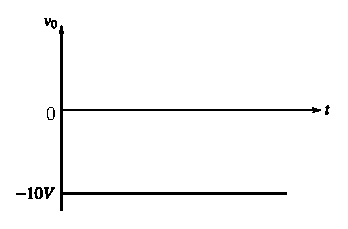
\includegraphics{chap4/sol4.26a.eps}}
\end{tabular}

~

\item[(b)]
\begin{tabular}[t]{c@{\hspace{3.8cm}}c}
\begin{tabular}[t]{@{}r@{\;}l}
$v_{i}\,$ & $= -5t\,\text{V}$\\[4pt]
$v_{0}$   & $= -\dfrac{d}{dt}[-5t]$\\[6pt]
          & $= 5\text{V}(DC)$
\end{tabular} & 
\raisebox{-1.8cm}{\includegraphics{chap4/sol4.26b.eps}}
\end{tabular}

~

\item[(c)]
\begin{tabular}[t]{c@{\hspace{3.8cm}}c}
\begin{tabular}[t]{@{}r@{\;}l}
$v_{i}\,$ & $= -2\,t^{2}\,\text{V}$\\[4pt]
$v_{0}$   & $= -\dfrac{d}{dt}[2t^{2}]$\\[6pt]
          & $= -4t\,\text{V}$
\end{tabular} & 
\raisebox{-1.8cm}{\includegraphics{chap4/sol4.26d.eps}}
\end{tabular}

~

\item[(d)]
\begin{tabular}[t]{c@{\hspace{3.1cm}}c}
\begin{tabular}[t]{@{}r@{\;}l}
$v_{i}\,$ & $= 2\cos 2t\,\text{V}$\\[4pt]
$v_{0}$   & $= -\dfrac{d}{dt}[2\cos 2t]$\\[6pt]
          & $= 4\sin 2t\,\text{V}$
\end{tabular} & 
\raisebox{-2.2cm}{\includegraphics{chap4/sol4.26c.eps}}
\end{tabular}
\end{itemize}
\vskip -.9cm
\end{solution}

\begin{example}\label{exam5.27}
For the circuit given below
\begin{itemize}
\item[(a)] Calculate the gain of amplifier $A_{1}$

\item[(b)] Calculate the gain of amplifier $A_{2}$

\item[(c)] Find the total gain

\item[(d)] Find $v_{01}$ and $v_{0}$ when $v_{i}=0.25\,\sin 10t\,\text{V}$
\end{itemize}
\begin{figure}[H]
\centering
\includegraphics{chap4/exp4.27.eps}
\end{figure}
\end{example}

\begin{solution}
\begin{itemize}
\item[(a)] Amplifier $A_{1}$ is configured as inverting amplifier
$$
A_{f_{1}}=-\dfrac{10\, k\Omega}{5\, k\Omega}=-2
$$

\item[(b)] Amplifier $A_{2}$ is configured as non-inverting amplifier
$$
A_{f_{2}}=1+\dfrac{20\, k\Omega}{10\, k\Omega}=3
$$

\item[(c)] Total gain is
\begin{align*}
A_{f} &= A_{f_{1}} \times A_{f_{2}}\\[4pt]
&= -2\times 3\\[4pt]
& =-6
\end{align*}

\item[(d)]
\begin{tabbing}
$v_{01}$  \= = $A_{f_{1}}v_{i}$\\[9pt]
         \> = $(-2)(0.25\sin 10t\,\text{V})$\\[9pt]
         \> = $-0.5\sin 10t\text{V}$\\[9pt]
$v_{02}$  \> = $A_{f_{2}}v_{o_1}$\\[9pt]
         \> = $(3)(-0.5\sin 10t\V)$\\[9pt]
         \> = $-1.5 \sin 10t\,\text{V}$
\end{tabbing}
\end{itemize}
\vskip -1cm
\end{solution}

\bigskip

\begin{example}%4.22
For the circuit shown below, write the expressions for output voltages $v_{A}$, $v_{B}$, $v_{C}$, and $v_{0}$.
\begin{figure}[H]
\centering
\includegraphics{chap4/exp4.28.eps}
\end{figure}
\end{example}

\begin{solution}
$A_{1}$ is configured as inverting amplifier
\begin{equation*}
\therefore\qquad v_{A}=-\left[\dfrac{1\,k\Omega}{1\,k\Omega}\right]v_{1}=-v_{1}\tag{A}
\end{equation*}
$A_{2}$ is configured as Integrator
\begin{align*}
\therefore\quad v_{B} &=-\dfrac{1}{(1\,M\Omega)(1\,\mu F)}\int\limits^{t}_{0}v_{2}\; dt\\[5pt]
\text{or}\qquad v_{B} &= -\int\limits^{t}_{0}v_{2}\; dt\tag{B}
\end{align*}
$A_{3}$ is configured as Differentiator.
\begin{align*}
\therefore\qquad v_{C} &=-(1\,M\Omega)(1\,\mu F)\dfrac{dv_{3}}{dt}\\[5pt]
\text{or}\qquad v_{C} &= -\dfrac{dv_{3}}{dt}\tag{C}
\end{align*}
$A_{4}$ is configured as summer, with inputs $v_{A}$, $v_{B}$ and $v_{C}$.
\begin{align*}
\therefore\qquad v_{0} &= -\left[\left(\dfrac{1\,k\Omega}{1\,k\Omega}\right)v_{A}+\left(\dfrac{1\,k\Omega}{1\,k\Omega}\right)v_{B}+\left(\dfrac{1\,k\Omega}{1\,k\Omega}\right)v_{C}\right]\\[5pt]
&= -\left[v_{A}+v_{B}+v_{C}\right]\tag{D}
\end{align*}
Substituting for $v_{A}$, $v_{B}$ and $v_{C}$ from equations (A), (B) and (C), we have
\begin{align*}
v_{0} &=-\left[-v_{1}-\int\limits^{t}_{0}v_{2}\;dt-\dfrac{d v_{3}}{dt}\right]\\[5pt]
\therefore\qquad v_{0} &= \left[v_{1}+\int\limits^{t}_{0}v_{2}\;dt+\dfrac{dv_{3}}{dt}\right]\tag{E}
\end{align*}
\end{solution}

\eject

\begin{example}%5.29
For the circuit shown below, calculate the output voltage $v_{0}$.
\begin{figure}[H]
\centering
\includegraphics{chap4/exp4.29.eps}
\end{figure}
\end{example}

\begin{solution}
The output $v_{0}$ can be calculated using superposition principle by applying the following steps.
\begin{description}
\item[Step 1~:] Reduce $v_{3}$ to zero and find the output due to $v_{1}$ and $v_{2}$. The resulting circuit is shown in Fig.~(A).
\begin{figure}[H]
\centering
\includegraphics{chap4/sol4.29a.eps}

\medskip
{\bf Fig.~A}
\end{figure}
\noindent
Observe that the non-inverting input terminal is grounded since, $v_{3}=0$.

\eject

The circuit of Fig.~(A) is an adder
\begin{align*}
\therefore\qquad v_{0_{1}} &= -\left[\left(\dfrac{20\,k\Omega}{10\,k\Omega}\right)v_{1}+\left(\dfrac{20\,k\Omega}{20\,k\Omega}\right)v_{2}\right]\\[5pt]
\text{or}\qquad v_{0_{1}} &= -[2v_{1}+v_{2}]\tag{A}
\end{align*}
Substituting for $v_{1}$ and $v_{2}$, we have
\begin{align*}
v_{0_{1}} &= -[2(-1\,V)+2\,V]\\[4pt]
\text{or}\qquad v_{0_{1}} &= 0\,V\tag{B}
\end{align*}

\item[Step 2~:] Reduce $v_{1}$ and $v_{2}$ to zero and find the output voltage due to $v_{3}$. The resulting circuit is shown in Fig.~(B).
\begin{figure}[H]
\centering
\includegraphics{chap4/sol4.29b.eps}

\smallskip
\medskip
{\bf Fig.~B}
\end{figure}

The circuit of Fig.~(B) is a non-inverting amplifier with input $v$. Also $10\,k\Omega$ and $20\,k\Omega$ are in parallel
\begin{equation*}
\therefore\qquad v_{0_{2}}=v\times \text{Gain}\tag{C}
\end{equation*}
using voltage division rule,
\begin{equation*}
v=\dfrac{v_{3}\times 10\,k\Omega}{10\,k\Omega+10\,k\Omega}=0.5\, v_{3}\tag{D}
\end{equation*}

The gain of non-inverting amplifier is
\begin{align*}
\text{Gain~} &= 1+\dfrac{20\,k\Omega}{10\,k\,\Omega\, \|\, 1020\,k\,\Omega}\\[4pt]
&= 4
\end{align*}

Now Eqn.~(C) becomes
\begin{align*}
v_{0_{2}} &= (0.5\,v_{3})\times 4\\[4pt]
&= 2v_{3}
\end{align*}
Substituting for $v_{3}$, we have
\begin{align*}
v_{0_{2}} &= 2\times 0.5\,\text{Sint}\, V\\[4pt]
&= \text{Sint~}V\tag{E}
\end{align*}

\item[Step 3~:] The output voltage is given by
$$
v_{0}=v_{0_{1}}+v_{0_{2}}
$$
Substituting for $v_{0_{1}}$ and $v_{0_{2}}$ from Eqns.~(B) and (E), we have
\begin{align*}
v_{0} &= 0\,V+\text{Sint~}V\\[4pt]
\text{or}\qquad v_{0} &=\text{Sint~}V\tag{F}
\end{align*}
\end{description}
\end{solution}

\begin{example}
With an example illustrate the necessity of an Op-amp to obtain the output voltage independent of load resistance.
\end{example}

\begin{solution}
Let it be required to add two signals $v_{1}$ and $v_{2}$. These two signals are applied to node `A' through resistors $R_{1}$ and $R_{2}$ as shown in Fig.~\ref{fig5.22}. The currents $i_{1}$ and $i_{2}$ produced by these signals are made to pass through $R_{0}$ to develop the sum voltage $v_{o}$. $R_{L}$ represents the load to which the sum voltage is applied.
\begin{figure}[H]
\centering
\includegraphics{chap4/sol4.27.eps}
\caption{Summing two signals using resistive network}\label{fig5.22}
\end{figure}
Applying Kirchhoff's Current Law at node $A$ we have
\begin{align*}
i_{1}+i_{2} &= i_{o}+i_{L}\tag{A}\\[7pt]
i_{1} &= \frac{v_{1}-v_{o}}{R_{1}}\\[3pt]
i_{2} &= \frac{v_{2}-v_{o}}{R_{2}}\\[3pt]
i_{o} &= \frac{v_{o}}{R_{o}}\\[3pt]
i_{L} &= \frac{v_{o}}{R_{L}}
\end{align*}
Using these relations in Eqn.~(A) we have
\begin{align*}
\frac{v_{1}-v_{o}}{R_{1}}+\frac{v_{2}-v_{o}}{R_{2}} &= \frac{v_{o}}{R_{o}}+\frac{v_{o}}{R_{2}}\\[3pt]
v_{0}\left[\frac{1}{R_{1}}+\frac{1}{R_{2}}+\frac{1}{R_{o}}+\frac{1}{R_{2}}\right] &= \frac{v_{1}}{R_{1}}+\frac{v_{2}}{R_{2}}\tag{B}
\end{align*}
Let
\begin{align*}
\frac{1}{R_{P}} &= \frac{1}{R_{o}}+\frac{1}{R_{L}}\tag{C}\\[3pt]
\therefore\quad R_{P} &= \frac{R_{o}R_{L}}{R_{0}+R_{L}}h\tag{D}
\end{align*}
$R_{P}$ is the parallel combination of $R_{o}$ and $R_{L}$.

\vfill\eject

Substituting Eqn.~(C) in Eqn.~(D) we have
$$
v_{o}\left[\frac{1}{R_{1}}+\frac{1}{R_{2}}+\frac{1}{R_{P}}\right]=\frac{v_{1}}{R_{1}}+\frac{v_{2}}{R_{2}}
$$

Multiplying both sides by $R_{P}$ we have
\begin{align*}
v_{o}\left[1+\frac{R_{P}}{R_{1}}+\frac{R_{P}}{R_{2}}\right] &= v_{1}[R_{P}/R_{1}]+v_{2}[R_{P}/R_{2}]\\[3pt]
v_{o} &= \frac{v[R_{P}/R_{1}]+v_{2}[R_{P}/R_{2}]}{[1+R_{P}/R_{1}+R_{P}/R_{2}]}\tag{E}
\end{align*}
From Eqn.~(E) we find that $v_{o}$ depends on $R_{P}$ which in turn depends on $R_{L}$. We want $v_{o}$ to be independent of $R_{L}$. This is possible if $R_{o}\ll R_{L}$ or $1/R_{o}\gg 1/R_{L}$.

From Eqn.~(C) we find that
\begin{align*}
\frac{1}{R_{P}} & \simeq \dfrac{1}{R_{o}}\\[3pt]
\text{or}\qquad R_{P} &= R_{o}
\end{align*}
Note that $R_{P}$ is small and independent of $R_{L}$. But this small value of $R_{P}$ results in small value of $v_{o}$ which is undesirable. Therefore it is necessary to use amplifier whose gain is independent of $R_{L}$. The Op-amp is well suited for this application since its closed loop voltage gain is independent of $R_{L}$ and depends only external resistors $R_{f}$ and $R_{1}$.
\end{solution}


\smallskip
\begin{center}
\rule{5cm}{1pt}\\[-2pt]
{\bf Exercise Problems}\\[-4pt]
\rule{5cm}{1pt}
\end{center}

\begin{enumerate}
\renewcommand{\labelenumi}{\bf\theenumi.}
\item For the circuit shown calculate the following
\begin{figure}[H]
\centering
\includegraphics{addfig/exr5.1.eps}
\end{figure}
\begin{itemize}
\item[(a)] Voltage gain

\vskip .15cm
\item[(b)] Input impedance

\vskip .15cm
\item[(c)] Output voltage $v_{0}$ if $v_{i}=20\sin \omega t$\,mV
\end{itemize}

\item For the circuit shown below calculate the following
\begin{itemize}
\item[(a)] Voltage gain

\vskip .15cm
\item[(b)] Output voltage $v_{0}$ if $v_{i}=50\sin \omega t$\,mV
\end{itemize}
\medskip
\begin{figure}[H]
\centering
\includegraphics{addfig/exr5.2.eps}
\end{figure}

\smallskip
\item For the circuit shown below, calculate the output voltage $v_{0}$.
\smallskip
\begin{figure}[H]
\centering
\includegraphics[scale=.9]{addfig/exr5.3.eps}
\end{figure}

\eject

\item Identify the following circuit and find the output voltage $v_{0}$.
\begin{figure}[H]
\centering
\includegraphics[scale=.9]{addfig/exr5.4.eps}
\end{figure}

\item Identify the following circuit and sketch the output voltage $v_{0}$.
\begin{figure}[H]
\centering
\includegraphics[scale=.9]{addfig/exr5.5.eps}
\end{figure}

\item In the circuit of $Q(5)$ Resistor and capacitor are interchanged. What operation the circuit performs. Sketch the output voltage if $v_{i}=2\cos 5t$\,V.
\end{enumerate}
